\section{Exploratory testing with Mamba}
The inductive biases and thoeretical capabilities of Mamba are an active area of
research. In this section we run a multitude of mini-experiments on the Mamba
architecture in order to understand it's capabilities better.
This section(and the background on SSMs and Mamba) constitute Maxwell's
independent portion. In this section, we attempt to recreate some

\subsection{Known Results For State-Space Models}
% SSMs are only able to model star-free languages
It is known that state space models are only capable of recognizing a subset of
the regular languages\cite{ssmformal}, called the star-free languages.
The authors define the star-free languages are as the languages that can be
defined with empty set, the empty string, individual symbols, concatenation, and
Boolean combinations.
One important subset of the star free languages is a language class that we will
denote $\SEARCH$.
\begin{definition}
    $\SEARCH$ is the class of all $\SEARCH_{s}$, where $\SEARCH_{s}$ is defined
    as the set of all strings containing $s$ as a substring.
\end{definition}
For instance, $\SEARCH_{\text{xyz}}$ is defined as $\Sigma^{*}xyz\Sigma^{*}$.
Mamba has been found to perform as well as transformers on finite n-gram
memorization tasks, but fails to generalize on multiple n-gram memorization
\cite{mambangram}.

\subsection{Star-Free Approximation with Mamba}
\begin{figure}
    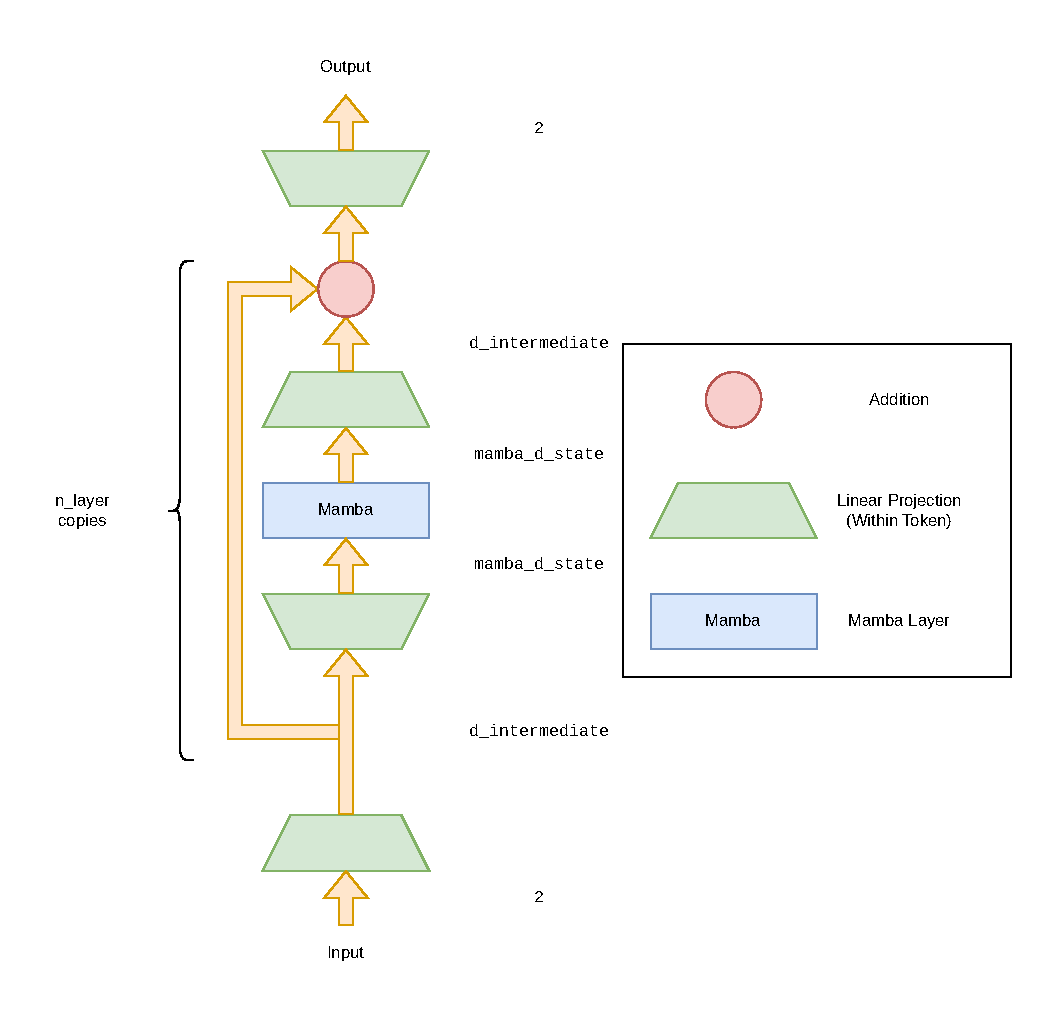
\includegraphics[width=\textwidth]{figures/sequence_stack_simple.pdf}
    \caption{Simple Mamba Stack Architecture}
    \label{simplestack}
\end{figure}

\begin{figure}
    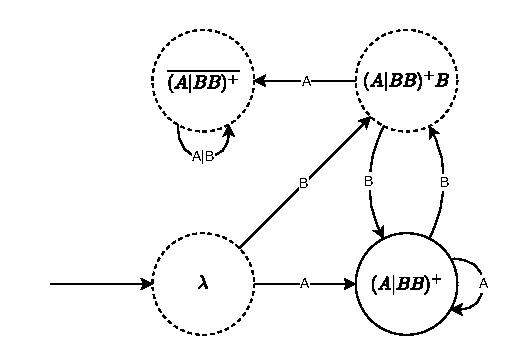
\includegraphics[width=\textwidth]{figures/a_or_bb_plus_dfa.pdf}
    \caption{DFA for \texttt{(a|bb)+}}
    \label{a_or_bb_plus_dfa}
\end{figure}


Despite their inability to perfectly predict non-star-free regular languages,
we find that Mamba is capable of recognizing certain non-star-free regular
languages with limited accuracy.

Preliminary testing on the regular language \texttt{(a|bb)+} shows a
surprisingly strong ability to recognize instances of the language, with lower
accuracy on medium-length strings.
If we construct the DFA for the language(see Figure \ref{a_or_bb_plus_dfa}), it
is clear that recognizing
the language requires recognizing odd-length runs of \verb|b|
We hypothesize that Mamba is searching for specific odd-length runs of \verb|b|.

\textbf{Dataset} The dataset that we train Mamba to recognize is a synthetic
dataset.
The instances are first randomly and uniformly assigned a length(from 1-64
inclusive) and a label(either in the language or not).
They are then randomly sampled given these constraints.
For instance, the data generator might first choose a length of 37, and a label
of true(in the language).
Then, it uniformly samples from the set of all length 37 strings in
\texttt{(a|bb)+}
The sampling is done with an efficient dynamic programming algorithm.

\textbf{Model} The model that we train is a stack of Mamba layers with linear
projection in-between(see Figure \ref{simplestack}).
The inputs and outputs also have linear projections to make the channel numbers
match the task.
The primary hyperparameters are \verb|n_layer = 2|, \verb|mamba_d_model = 16|,
and \verb|mamba_d_state = 16|.
The rest of the hyperparameters can be found on
Github\footnote{\url{https://github.com/maxwell3025/CV-IS-Fall-2024/blob/main/mamba_formal/config/experiment_a_or_bb.yaml}}.

\textbf{Results} 
\begin{figure}
    \begin{subfigure}{0.5\textwidth}
        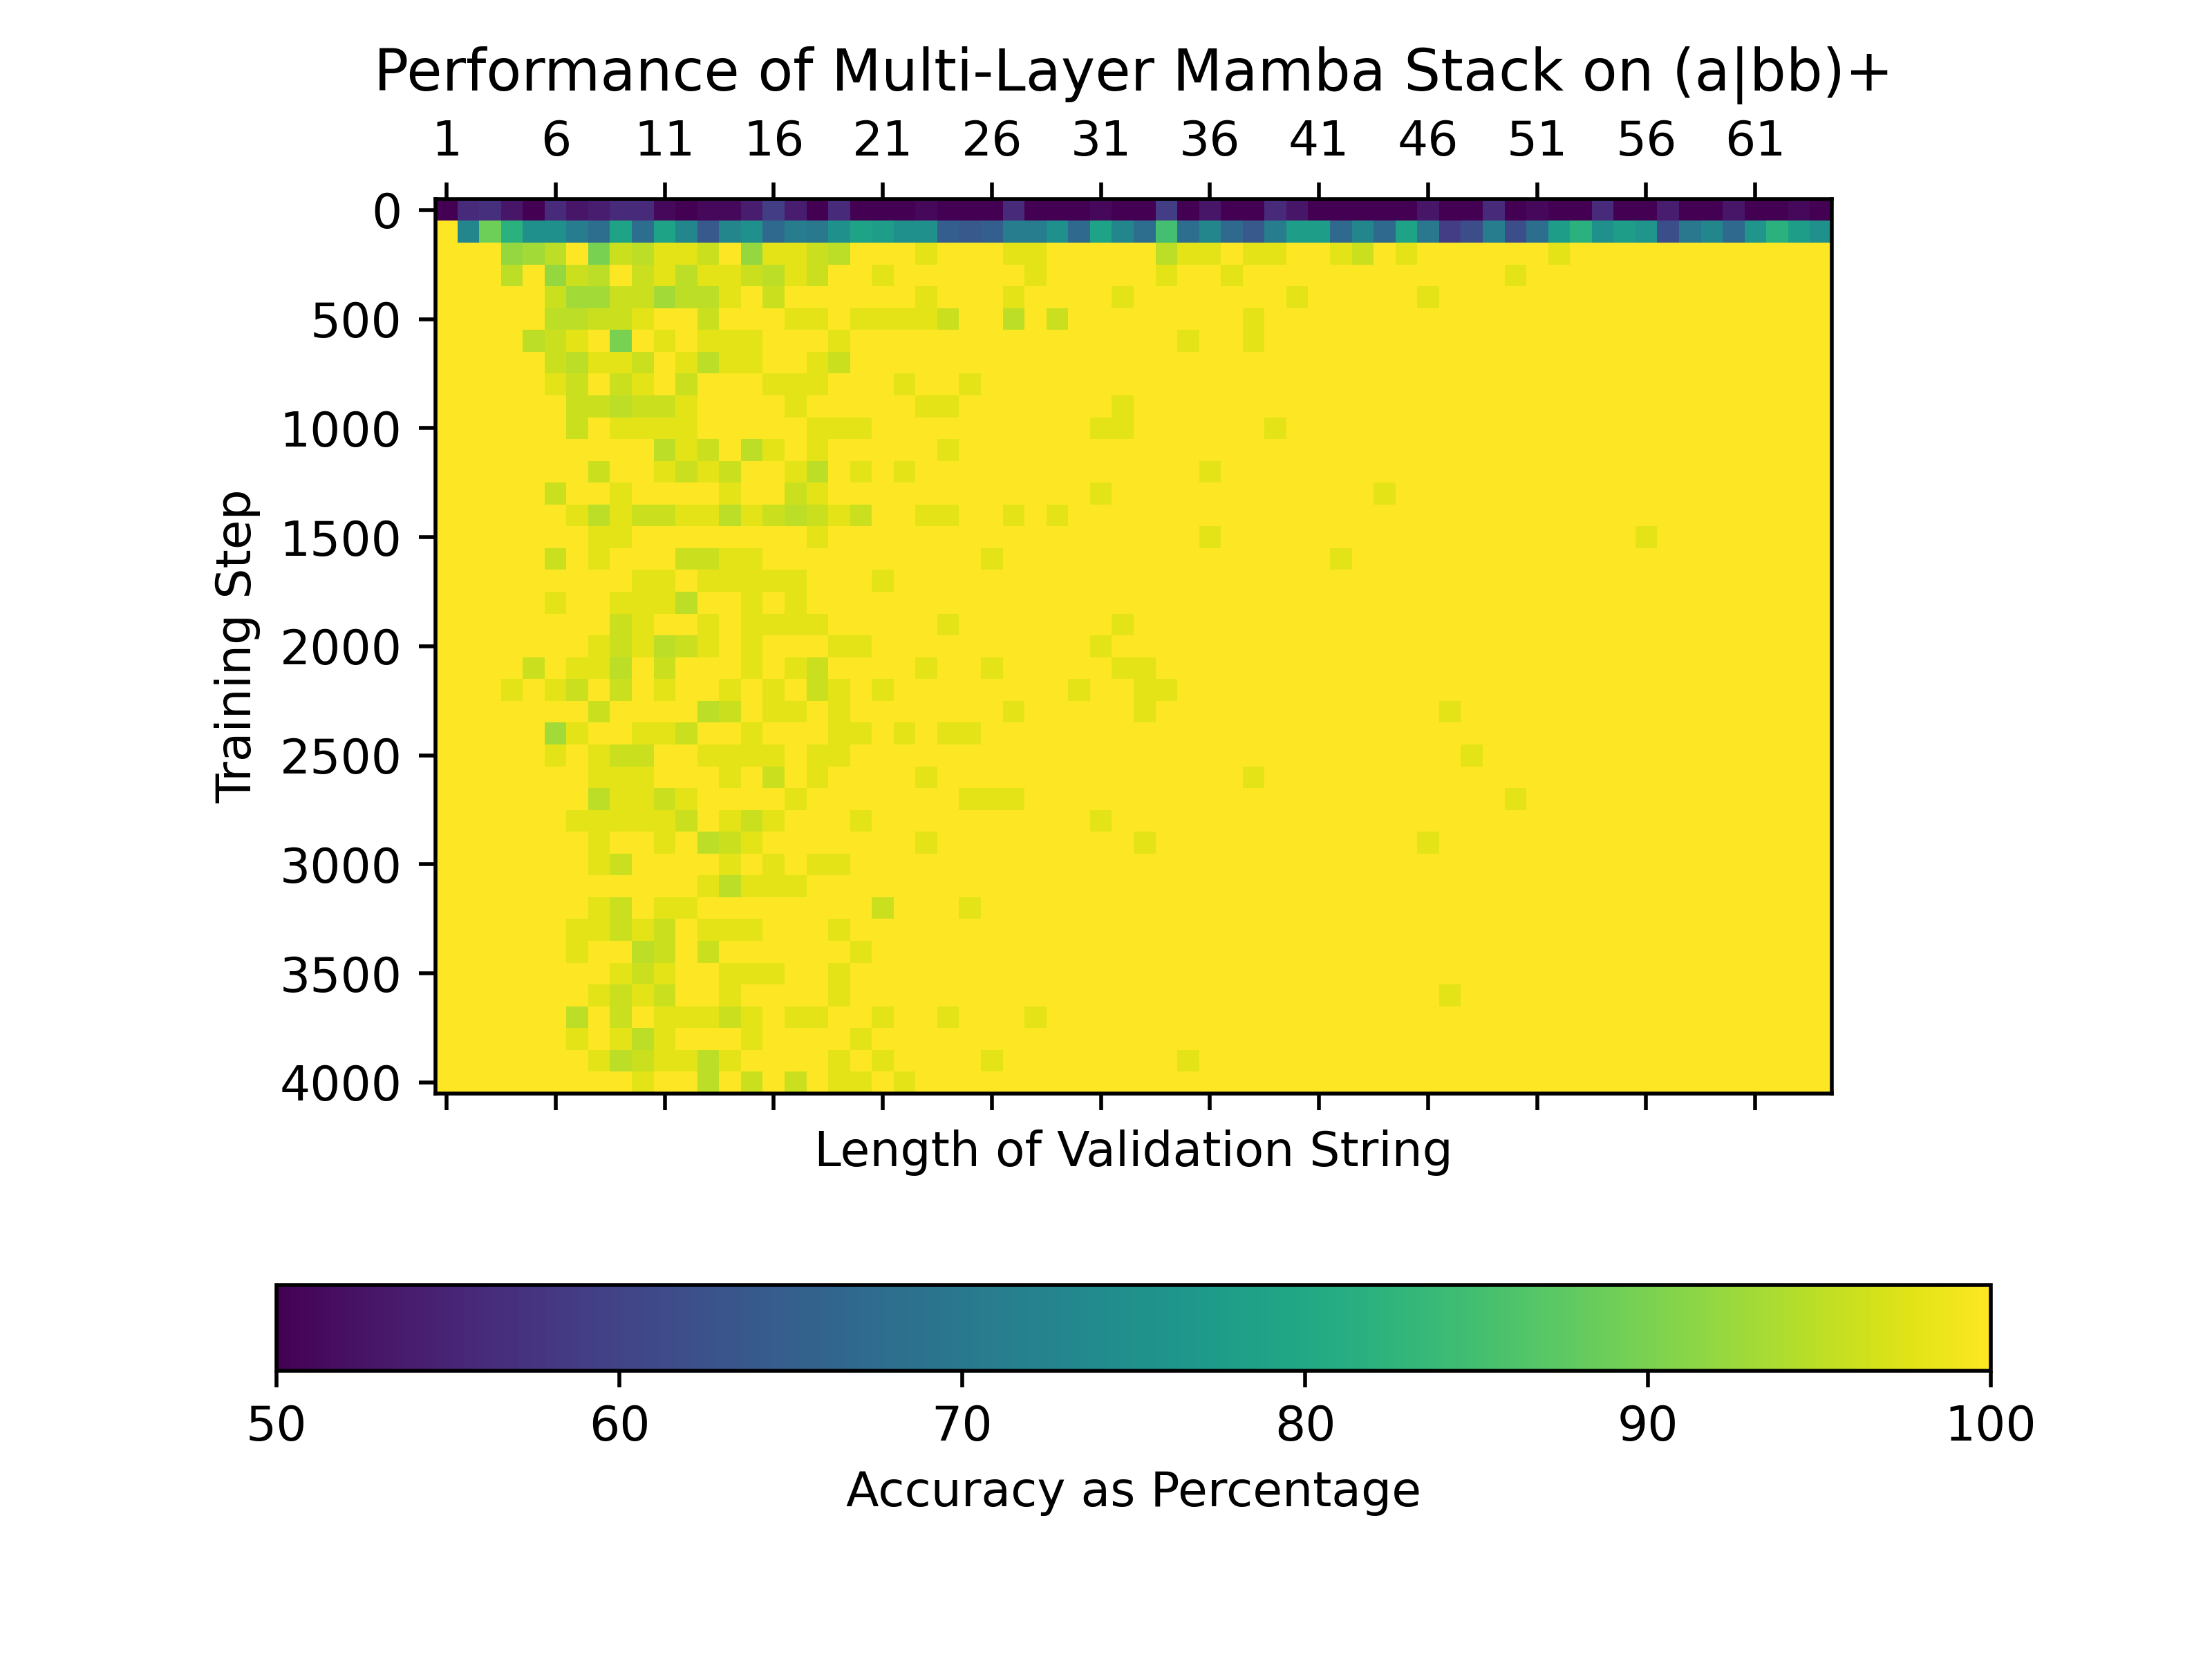
\includegraphics[width=\textwidth]{figures/a_or_bb_plus_mixed.png}
        \caption{}
    \end{subfigure}
    \begin{subfigure}{0.5\textwidth}
        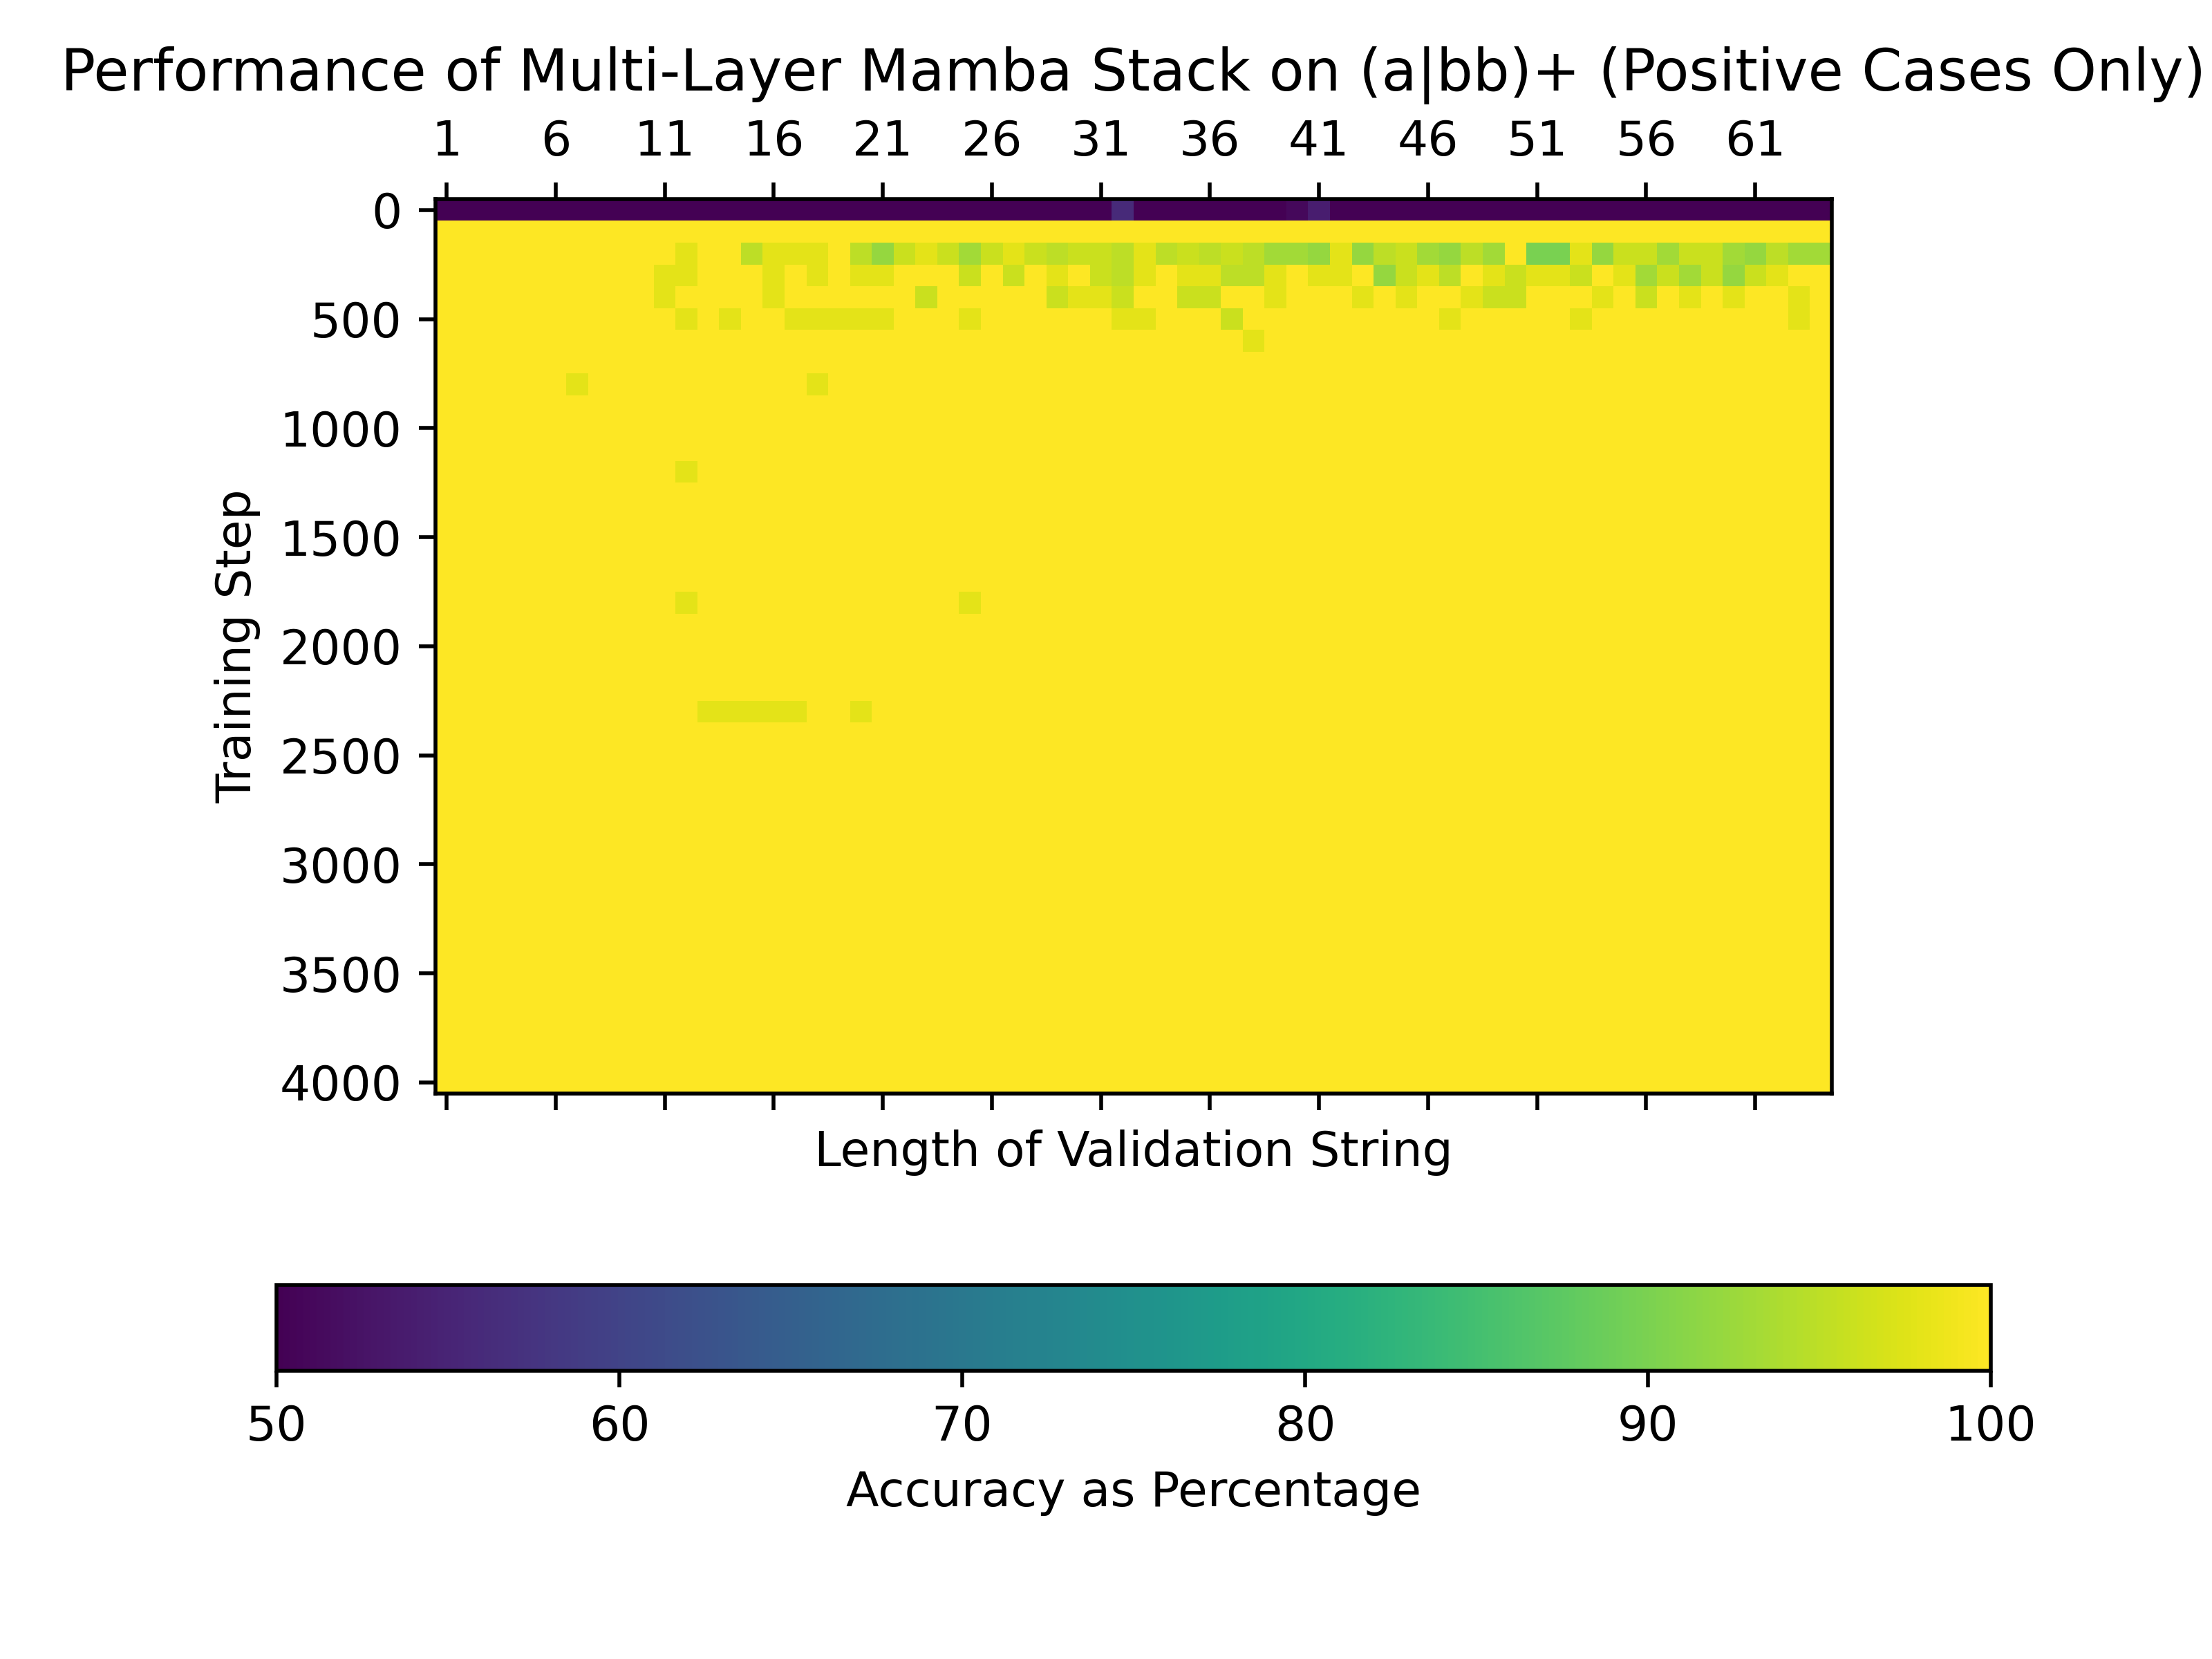
\includegraphics[width=\textwidth]{figures/a_or_bb_plus_positive_only.png}
        \caption{}
    \end{subfigure}
    \caption{Results for \texttt{a|bb+}}
\end{figure}
We find that the model quickly attains nearly perfect performance on positive
cases, with the trained model only making errors with negative cases.
This strongly suggests that our hypothesis is true.
The model is correctly identifying that positive cases lack the forbidden
strings that the model memorized, and the model is failing to recognize some
negative cases, since they contain odd-length forbidden strings that were not
memorized.

\subsection{Formation of "Bad Habits" with Mamba}
% Mamba interferes with LSTMs
Given Mamba's limited ability to recognize regular languages, it would be useful
to place it alongside more formally powerful models such as LSTMs, which can
trivially model general regular languages given large enough
parameters\cite{lstmformal}. Unfortunately, preliminary testing found that the
inclusion of Mamba in series with LSTMs leads to a degradation of generalization
ability.

We suspect that this explains the inclusion of drop-path in many ML
architectures.
Drop-path is a normalization layer introduced by FractalNet\cite{fractalnet} in
which the outputs of entire layers in an architecture are "zeroed-out".
As stated by the authors, this trains the model to do the task without certain
components.
In the literature, we find that machine learning architectures like
MedMamba\cite{medmamba}, VMamba\cite{vmamba}, and MambaND\cite{mamband} apply
drop-path to the output of Mamba layers.
We suspect this is done since Mamba learns certain tasks very quickly, leading to
the derivatives produced by Mamba to "drown out" the derivatives coming from the
other layers.
Drop-path would allow the other layers to then learn to solve the tasks without
being influenced by the Mamba layer.

In order to confirm these findings, we test a mixed Mamba model to solve a task
that Mamba alone cannot solve.

\textbf{Model} Our model in this test is identical to the model shown in
Figure \ref{simplestack}, except that 2 input layers are replaced with LSTM
layers.
In addition, drop path layers are placed after each Mamba layer.

\textbf{Dataset} We train our models to recognize even-length bitstrings.
It has been shown that Mamba cannot find parity\cite{ssmformal}, while parity
is a trivial task for LSTM architectures.

\textbf{Results}
\begin{figure}
    \begin{subfigure}{0.5\textwidth}
        \begin{center}
        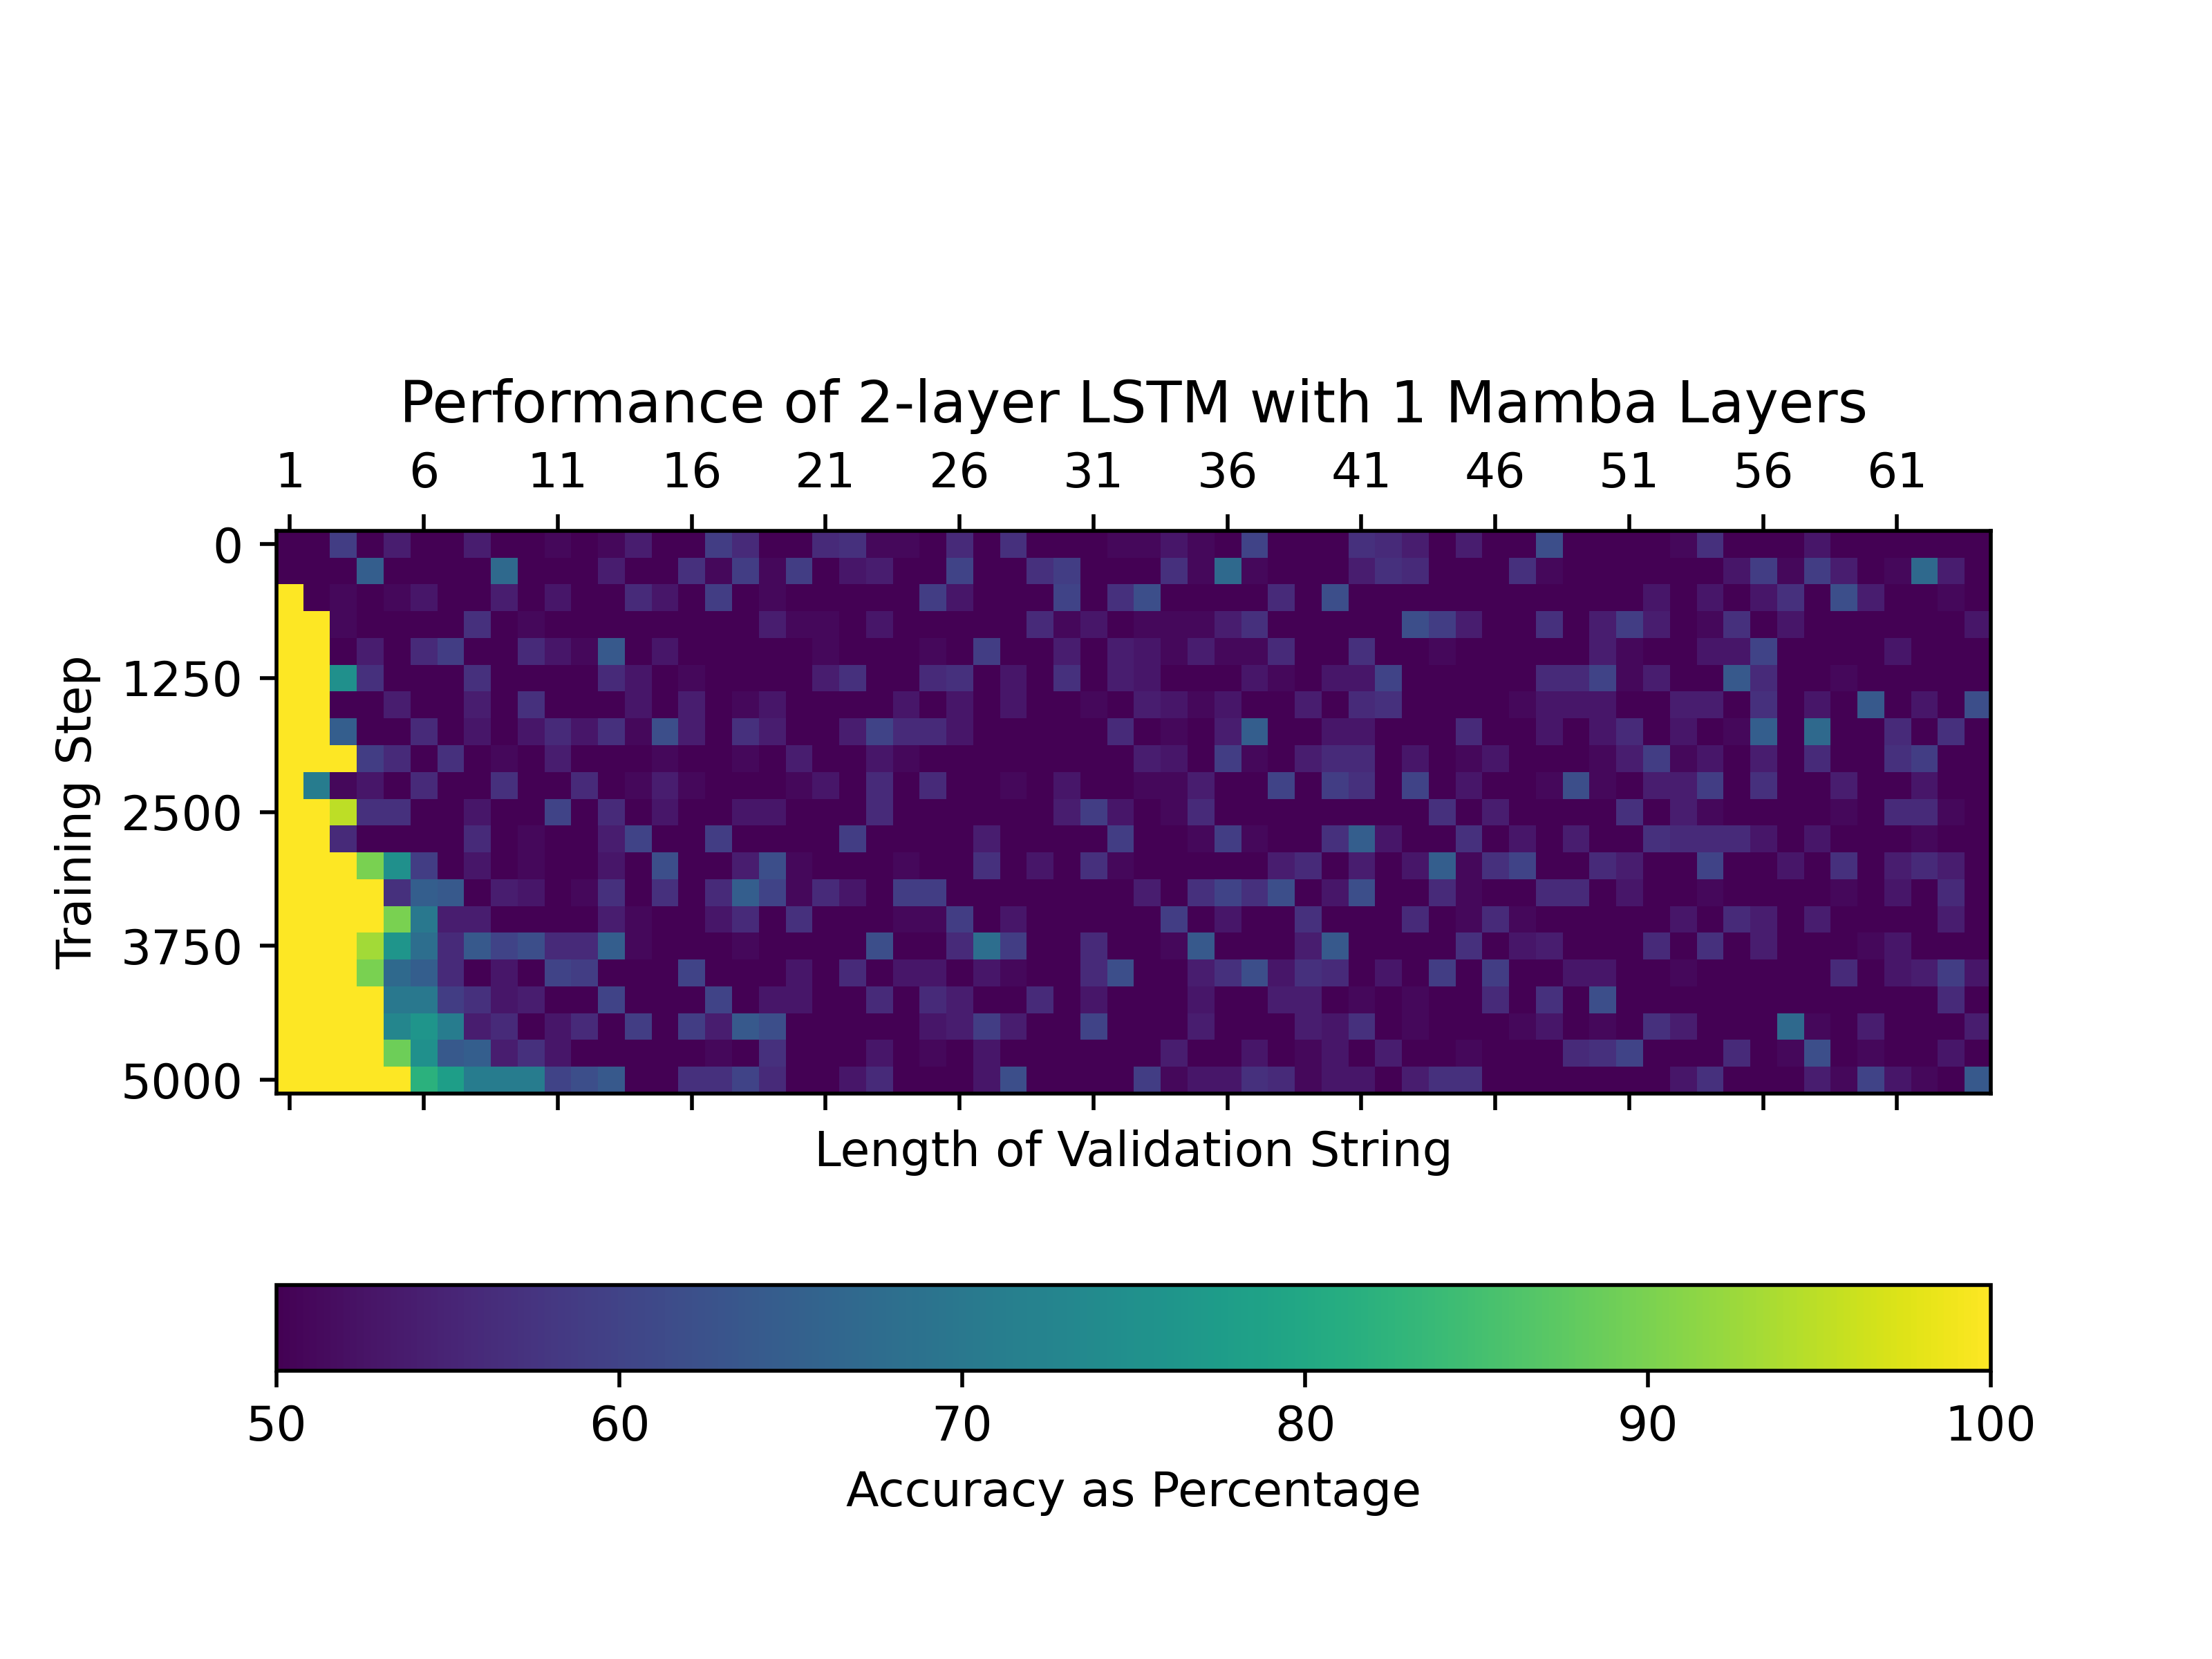
\includegraphics[width=0.8\textwidth]{figures/parity_lstm_False_3_1.png.png}
        \end{center}
    \end{subfigure}\begin{subfigure}{0.5\textwidth}
        \begin{center}
        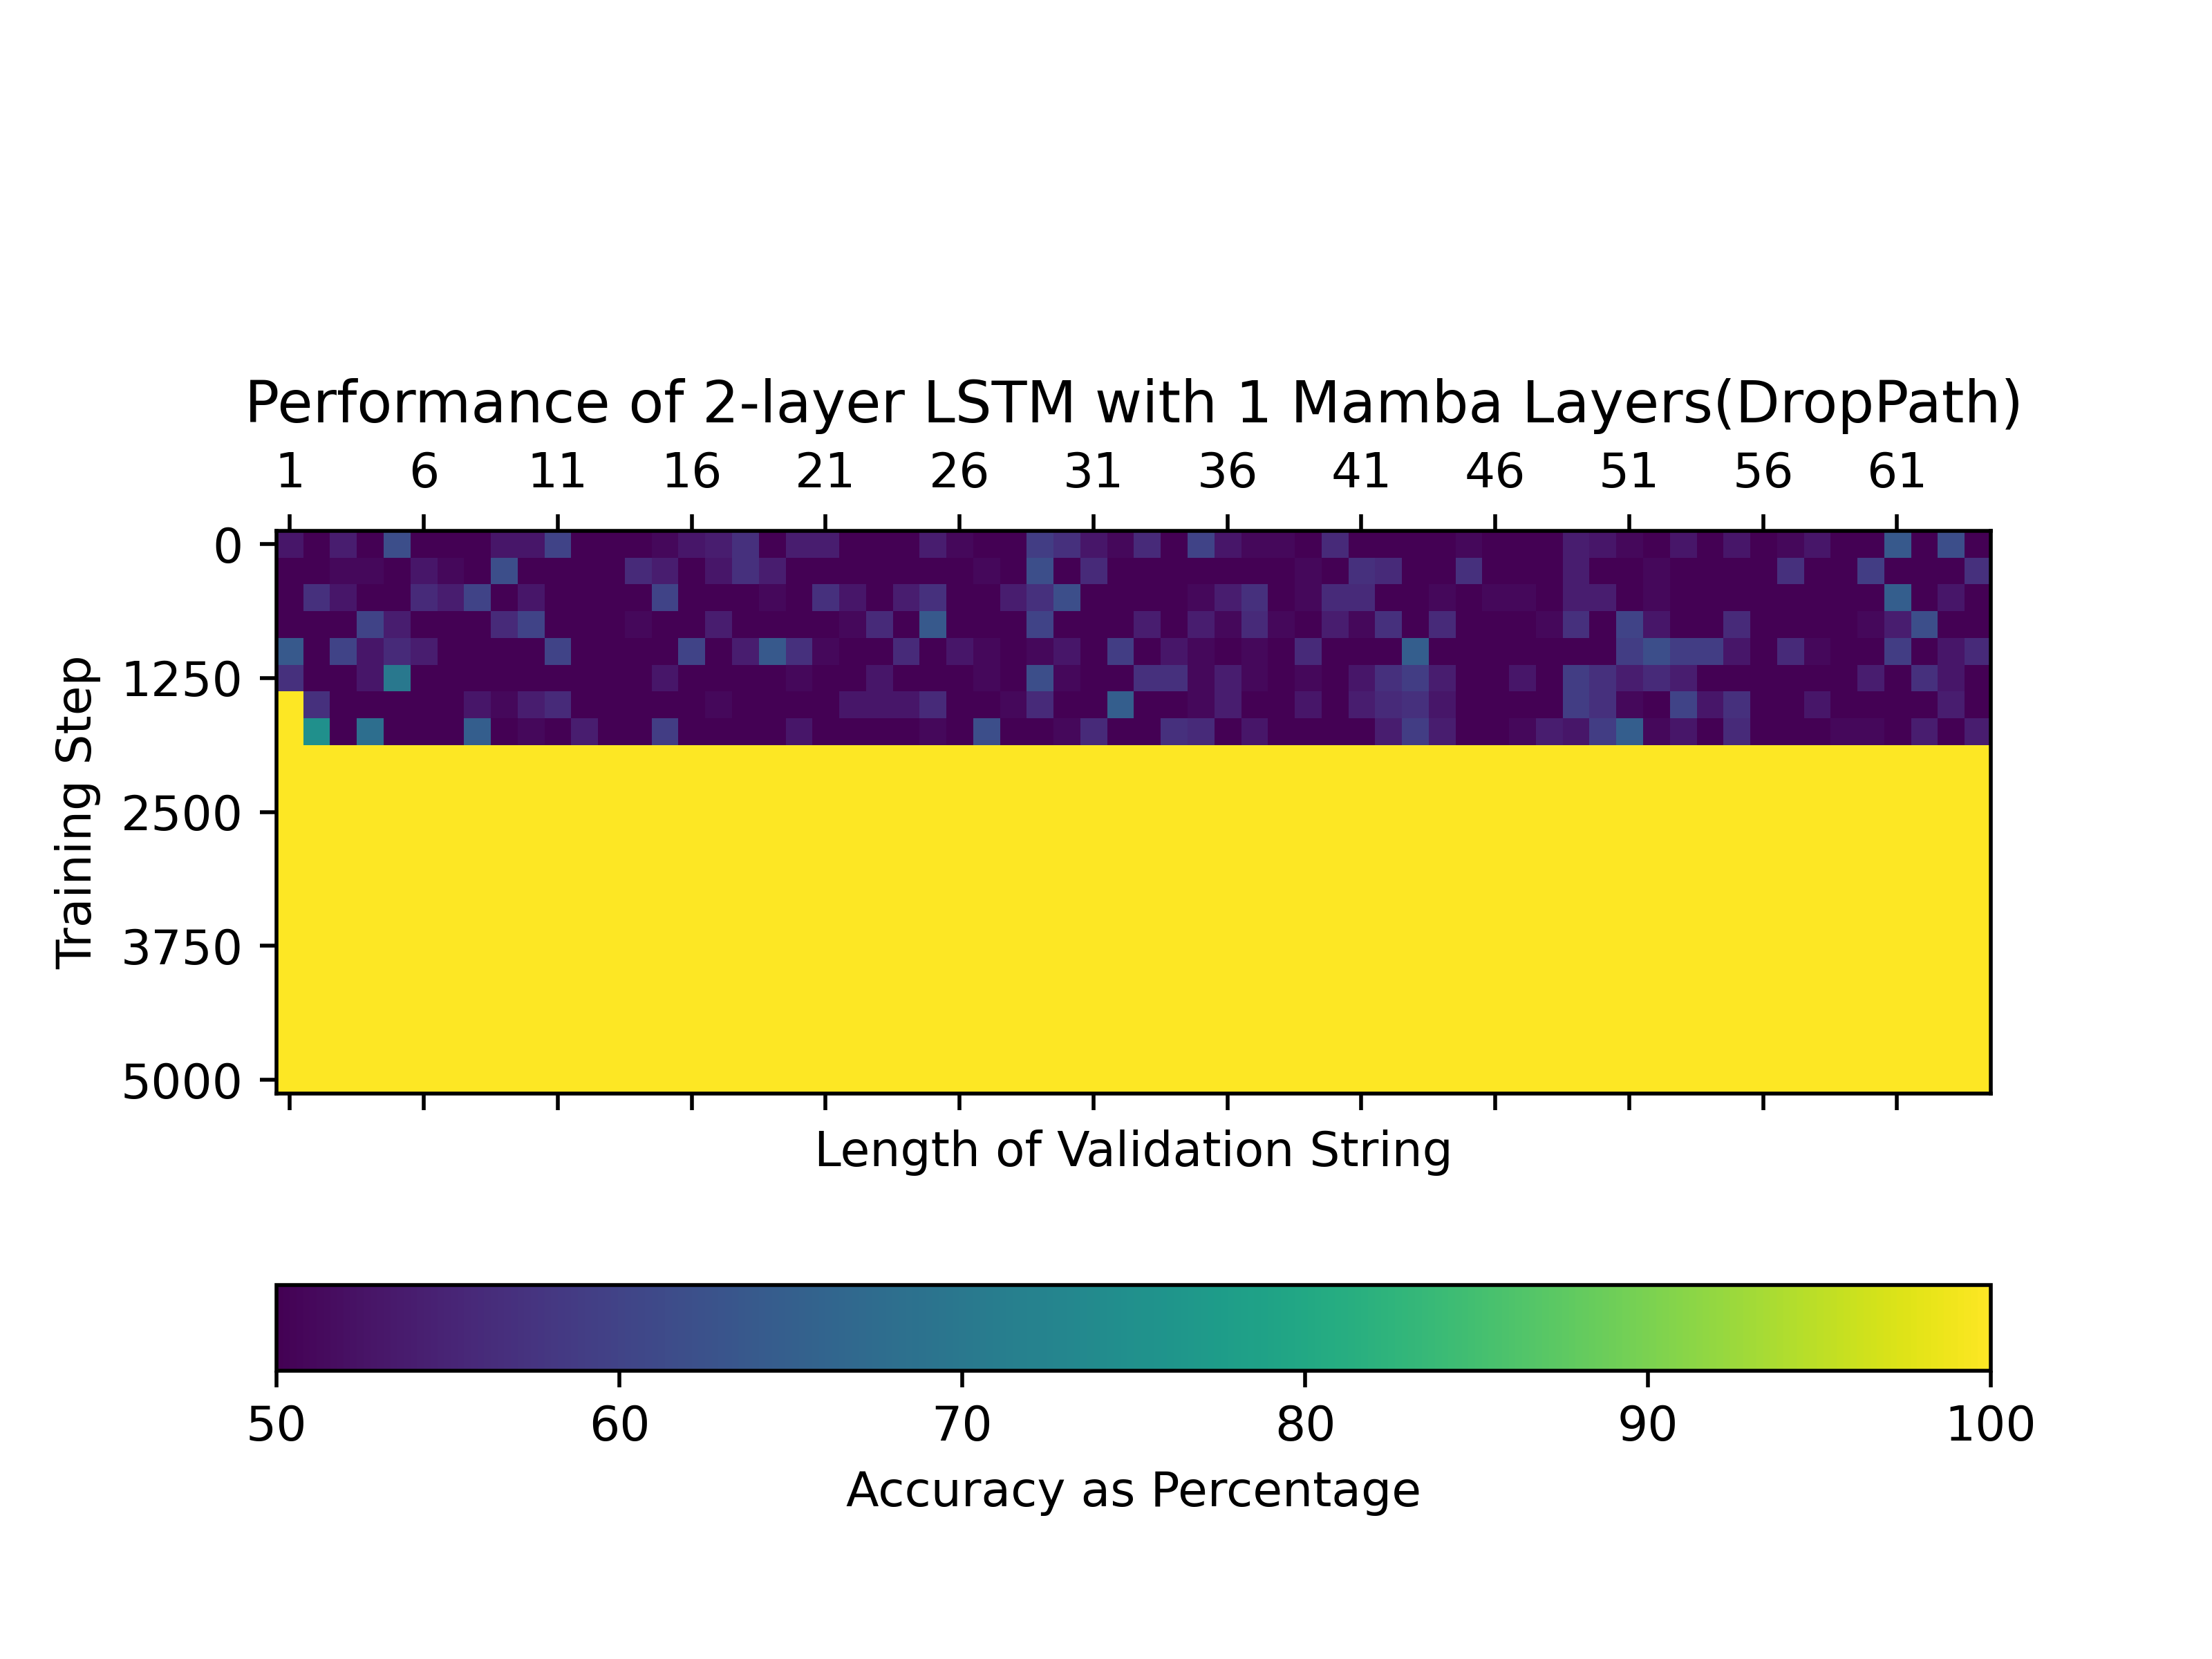
\includegraphics[width=0.8\textwidth]{figures/parity_lstm_True_3_1.png.png}
        \end{center}
    \end{subfigure}
    \begin{subfigure}{0.5\textwidth}
        \begin{center}
        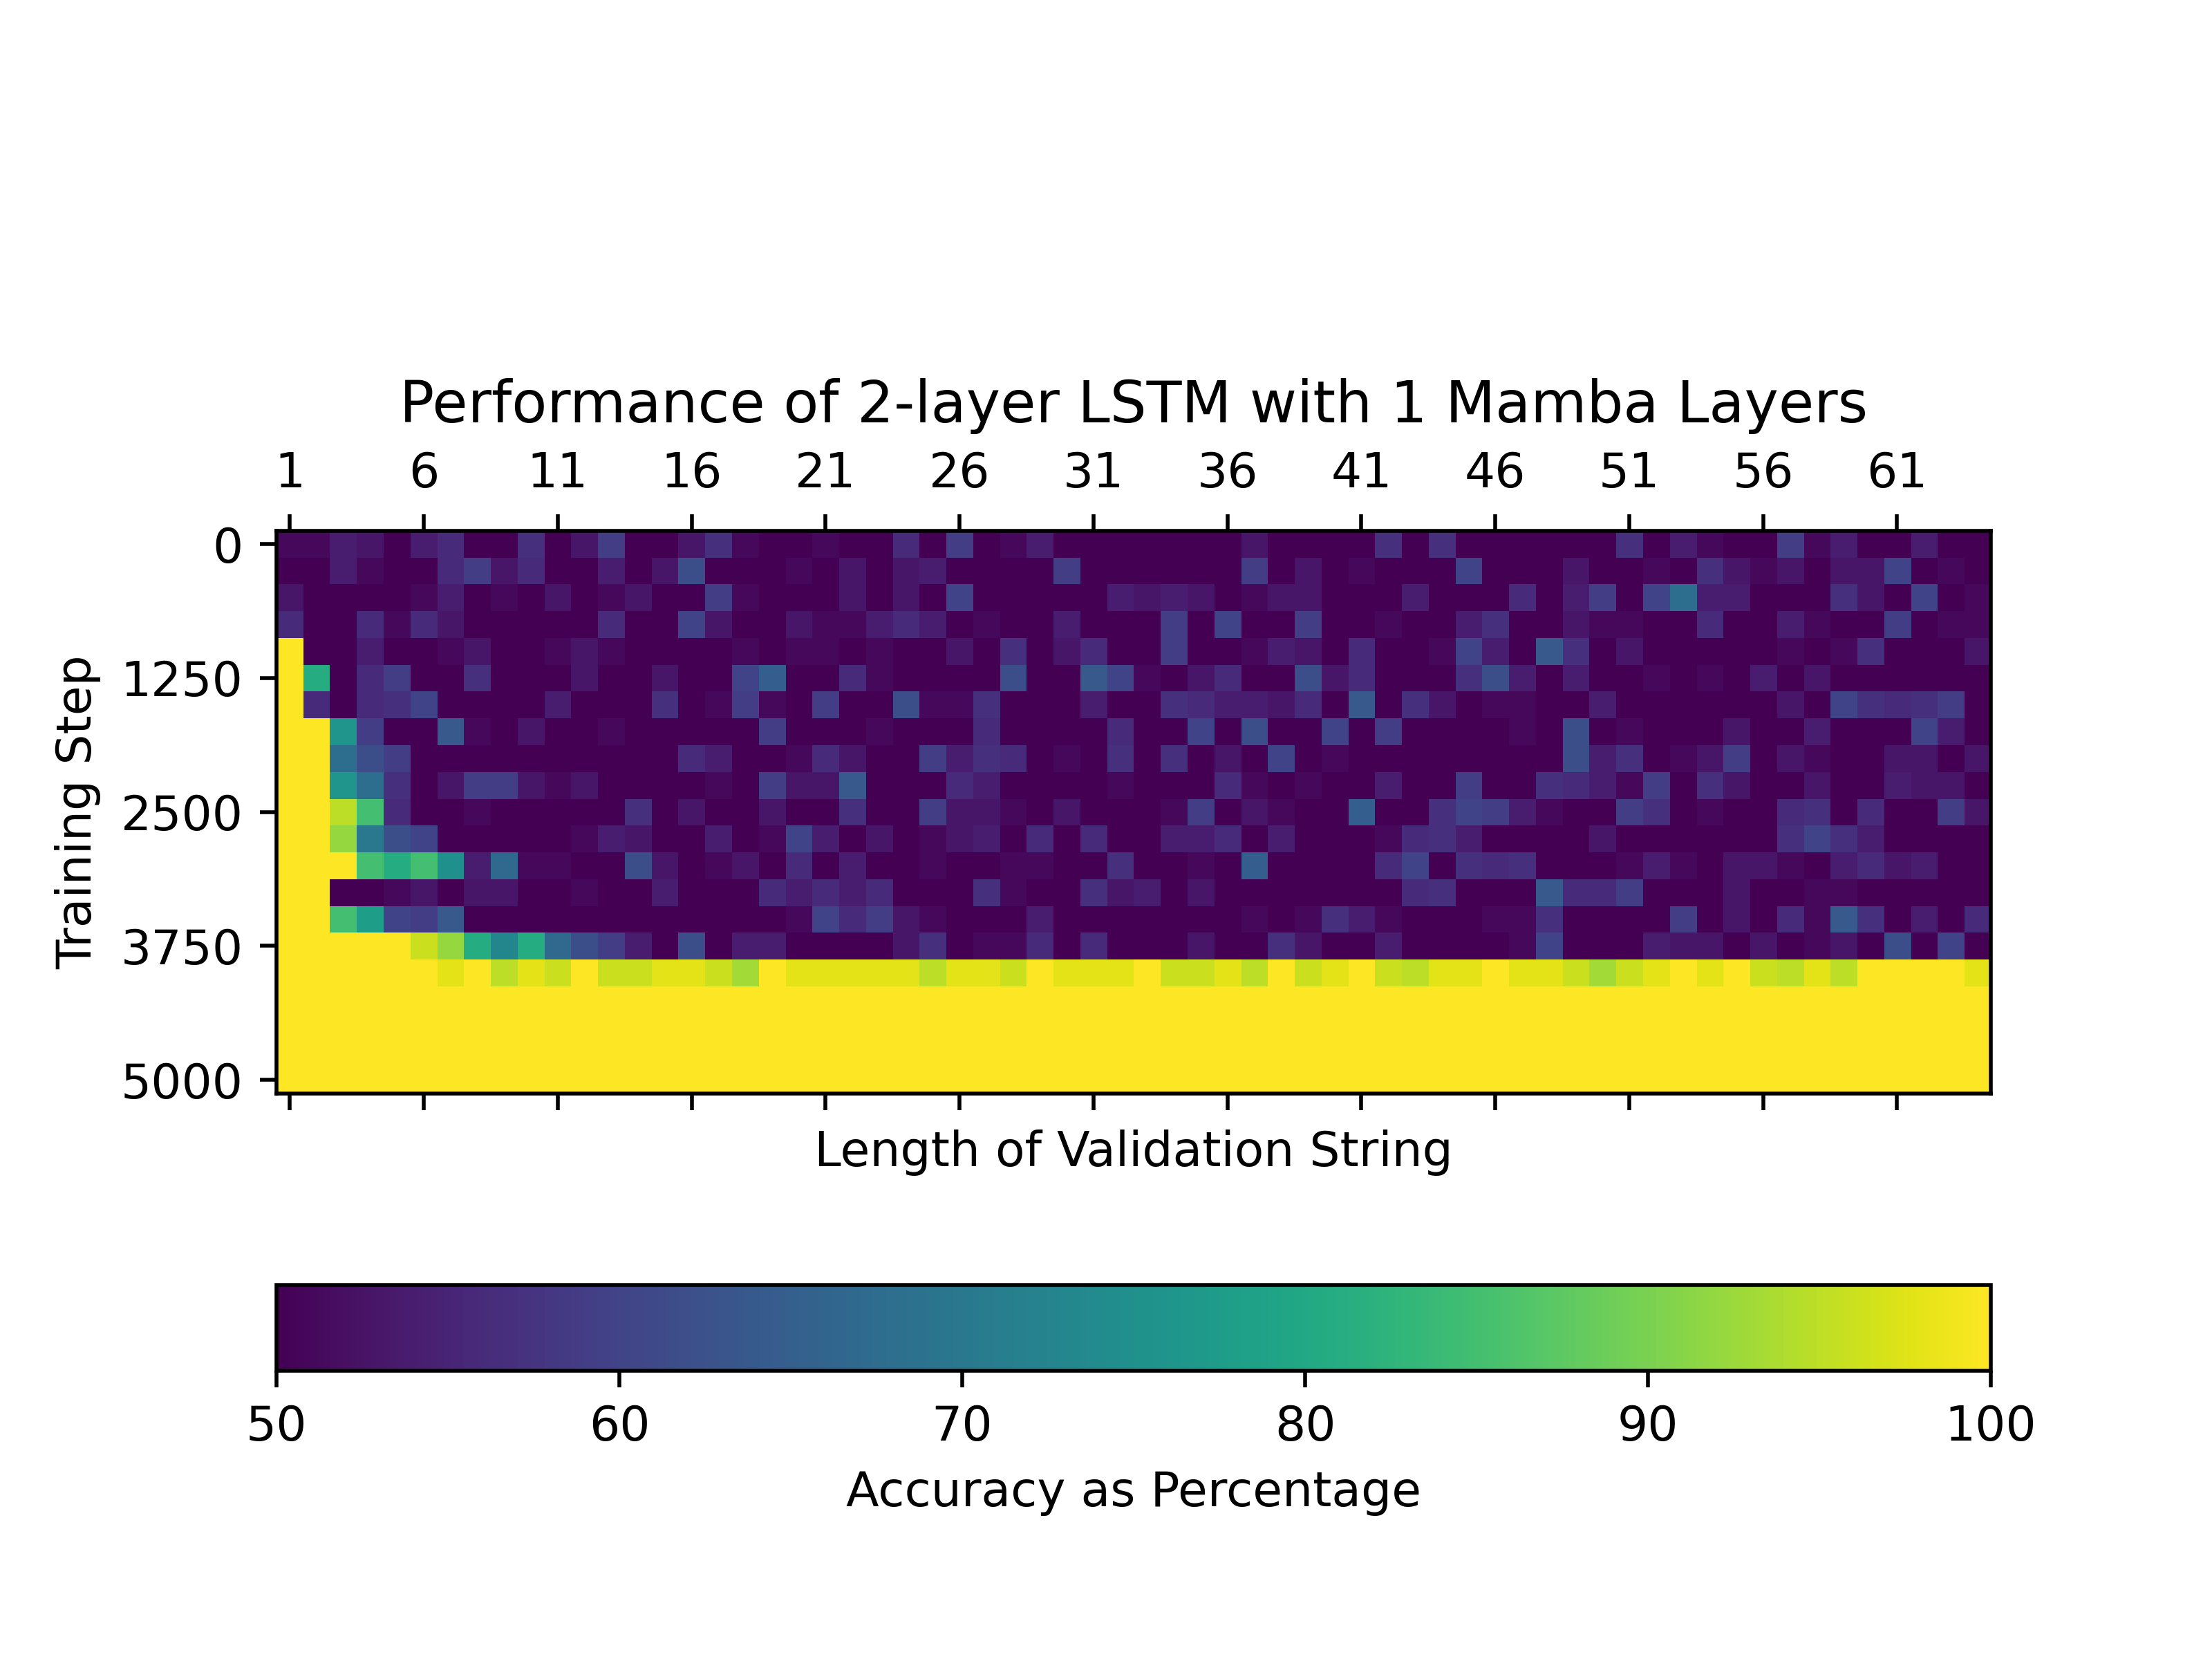
\includegraphics[width=0.8\textwidth]{figures/parity_lstm_False_3_2.png.png}
        \end{center}
    \end{subfigure}\begin{subfigure}{0.5\textwidth}
        \begin{center}
        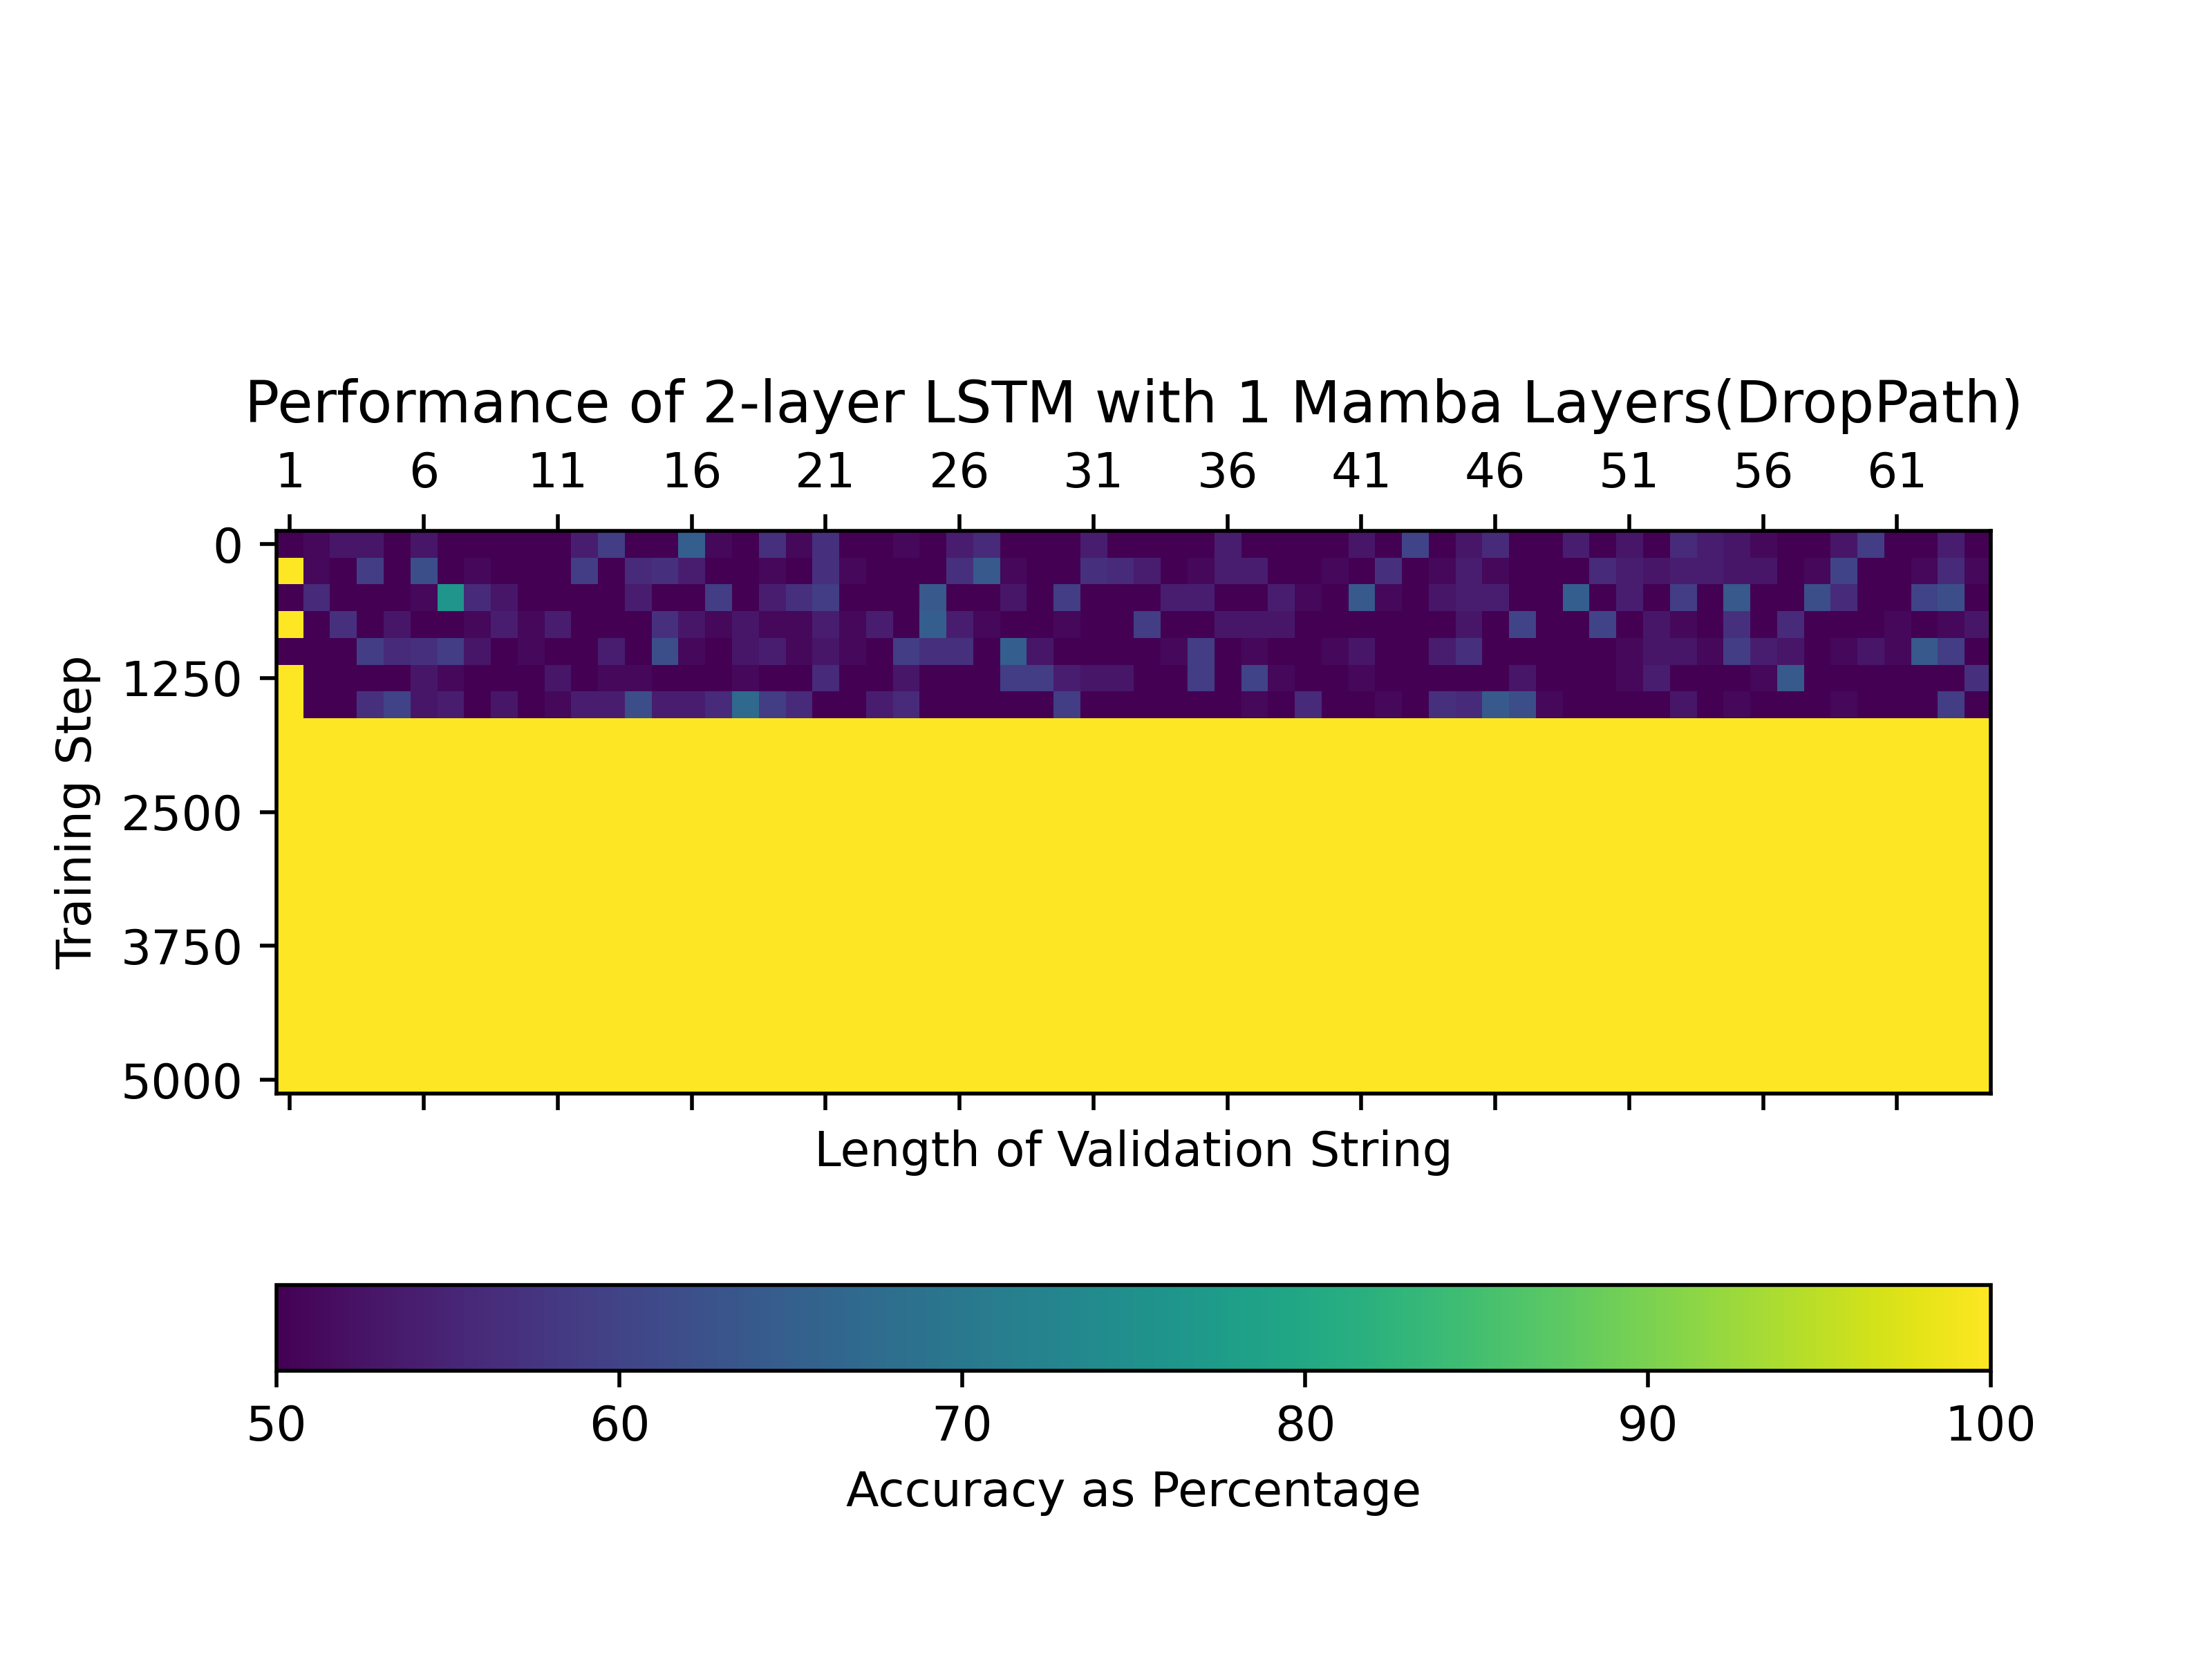
\includegraphics[width=0.8\textwidth]{figures/parity_lstm_True_3_2.png.png}
        \end{center}
    \end{subfigure}
    \begin{subfigure}{0.5\textwidth}
        \begin{center}
        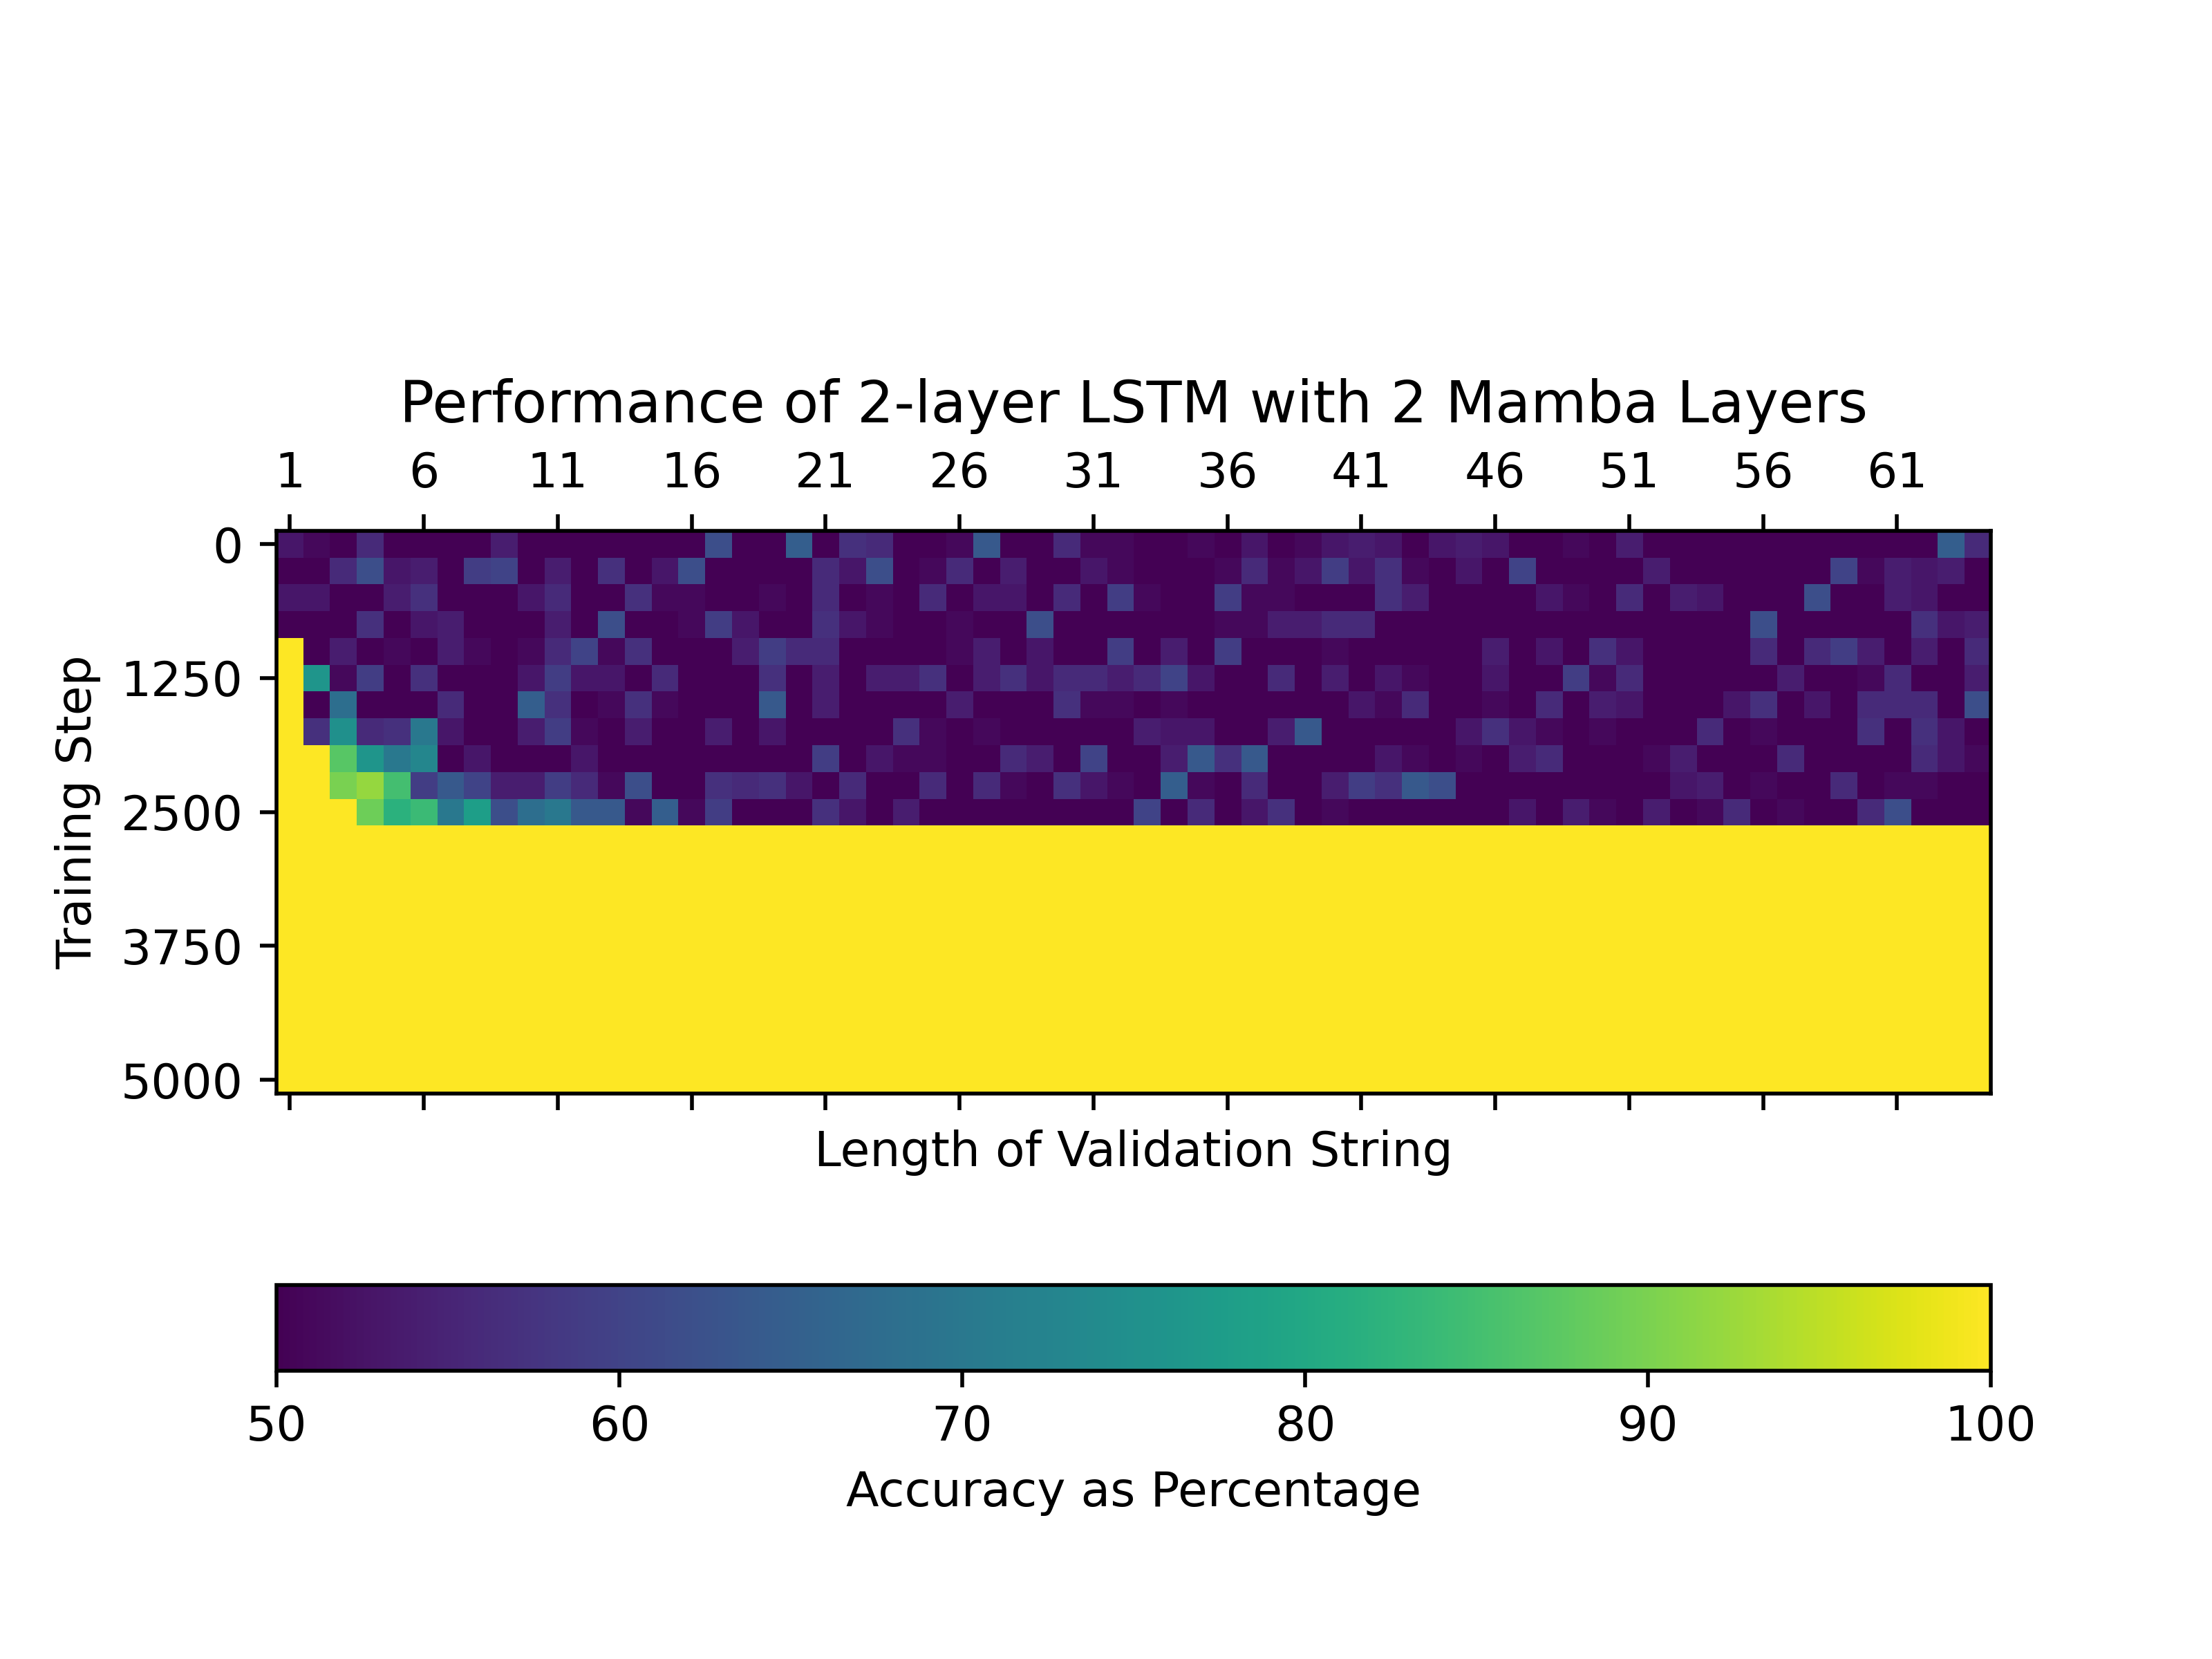
\includegraphics[width=0.8\textwidth]{figures/parity_lstm_False_4_1.png.png}
        \end{center}
    \end{subfigure}\begin{subfigure}{0.5\textwidth}
        \begin{center}
        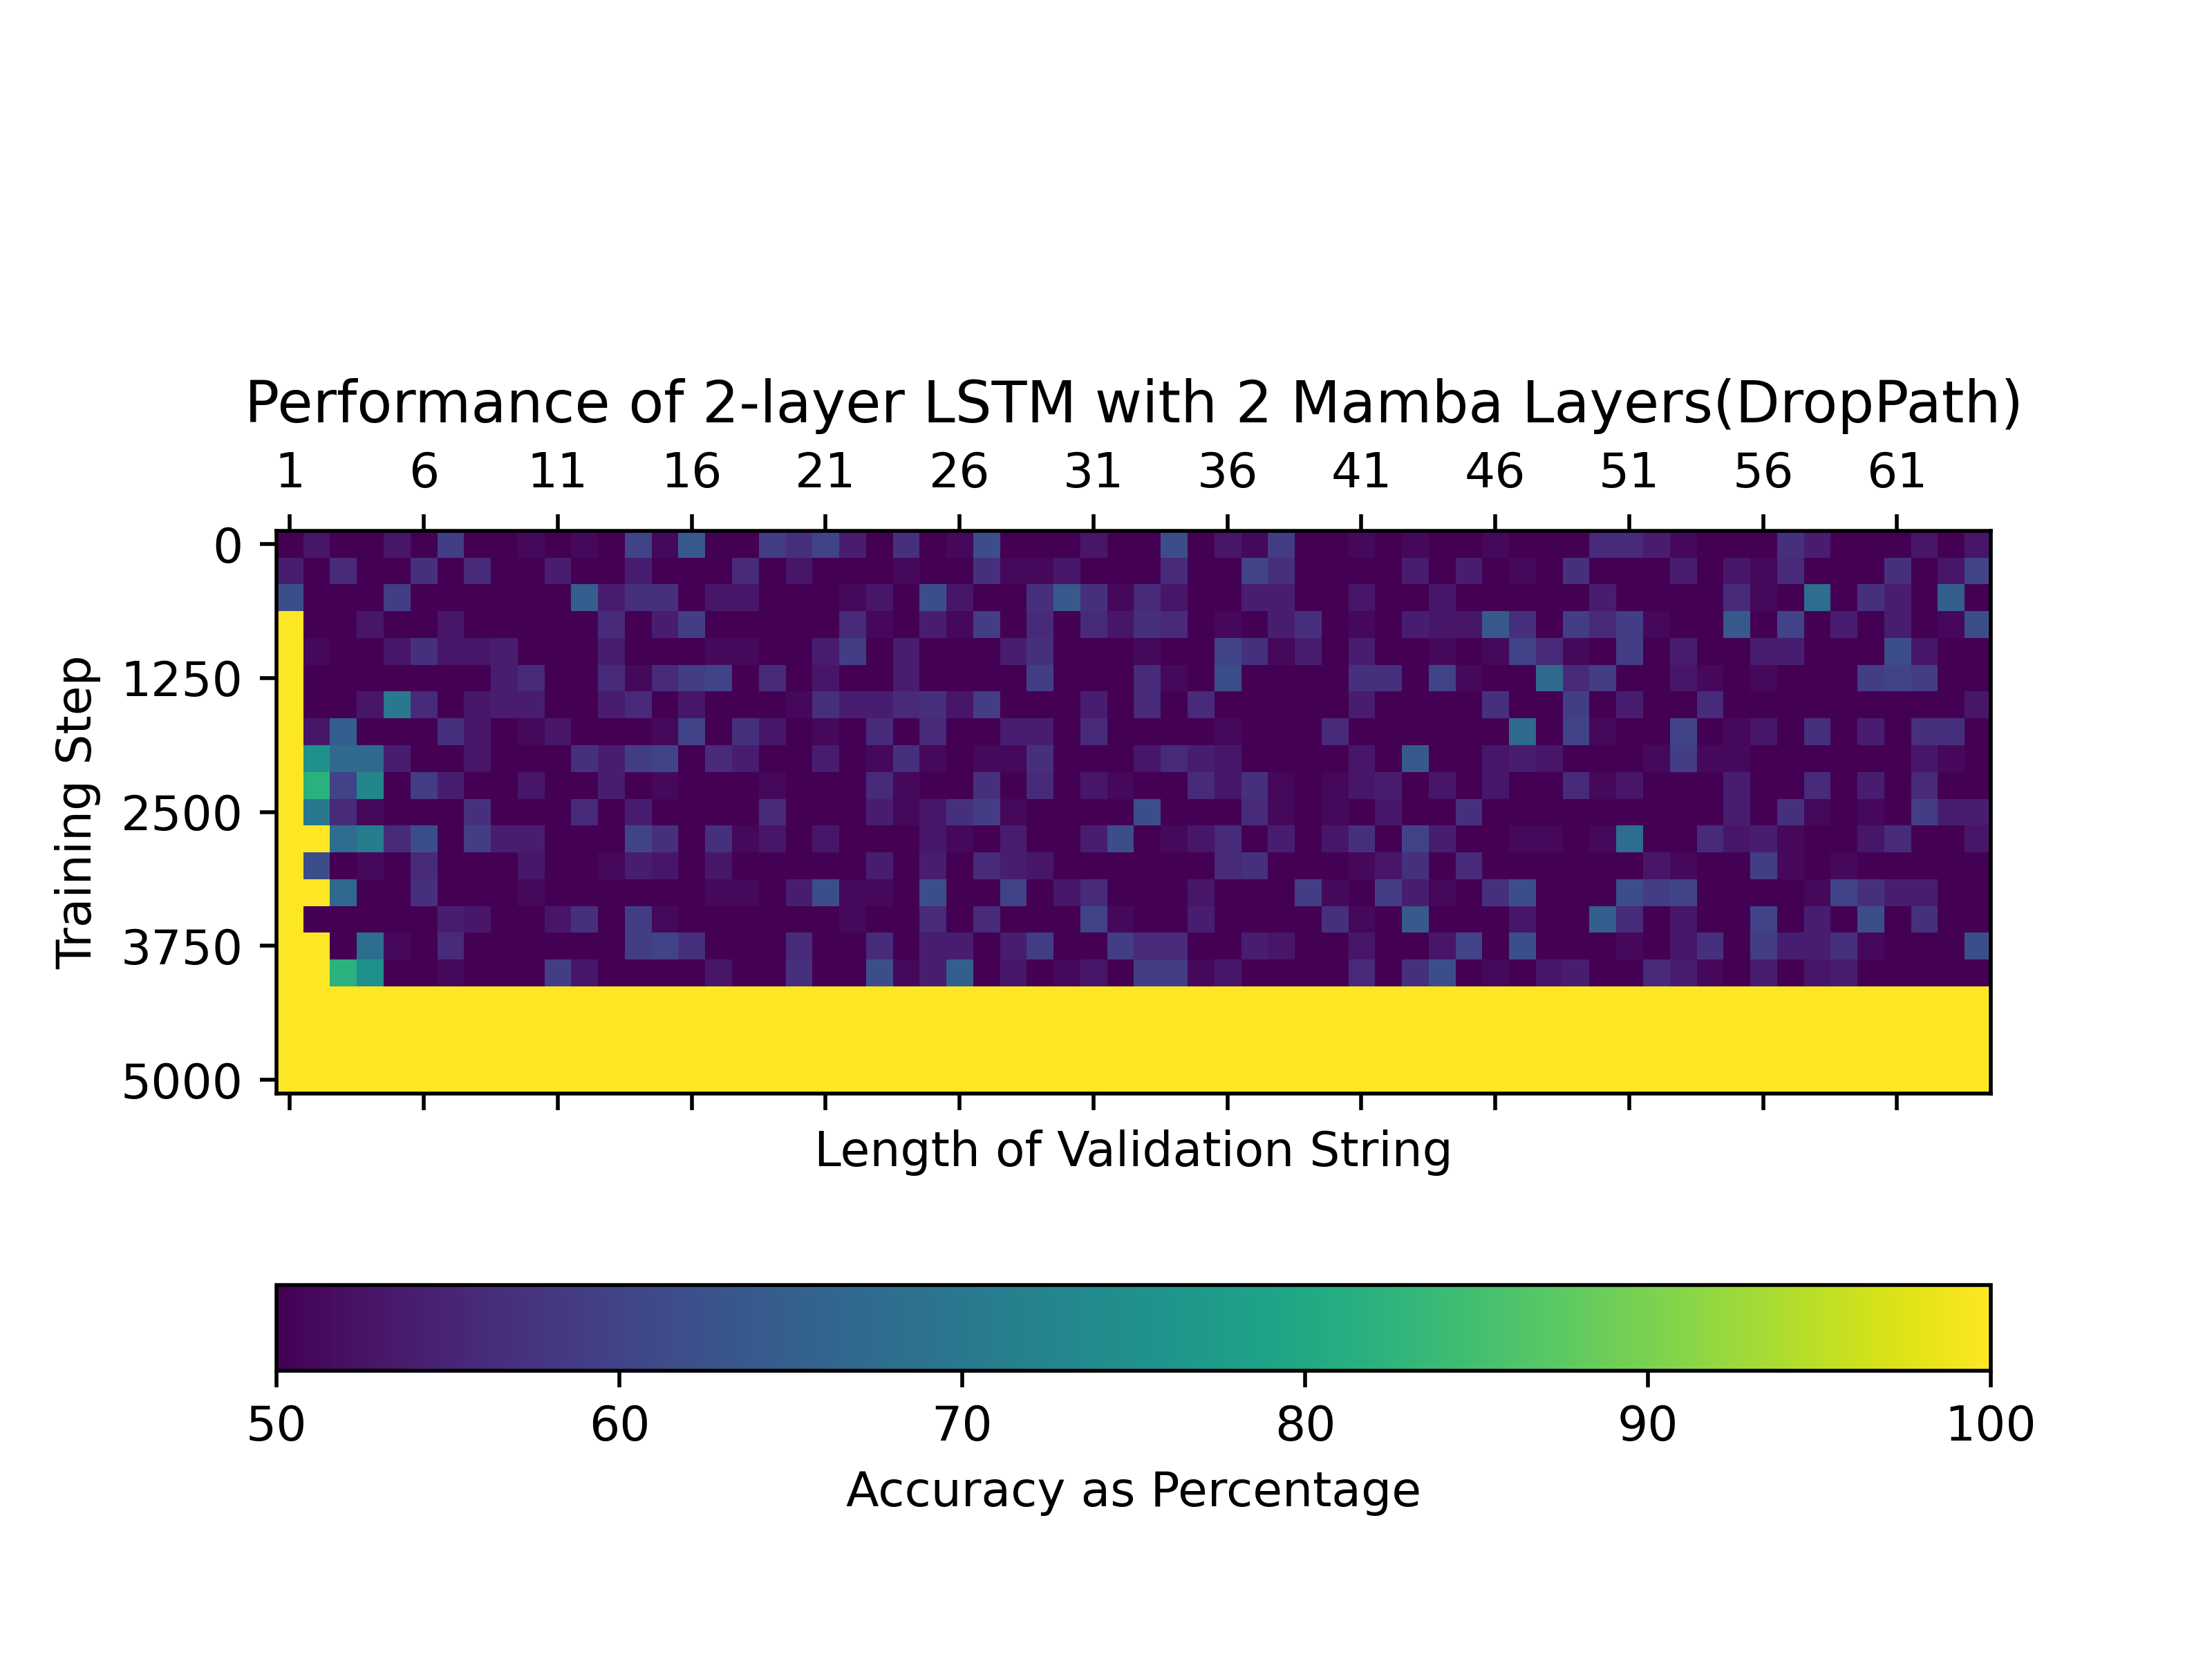
\includegraphics[width=0.8\textwidth]{figures/parity_lstm_True_4_1.png.png}
        \end{center}
    \end{subfigure}
    \begin{subfigure}{0.5\textwidth}
        \begin{center}
        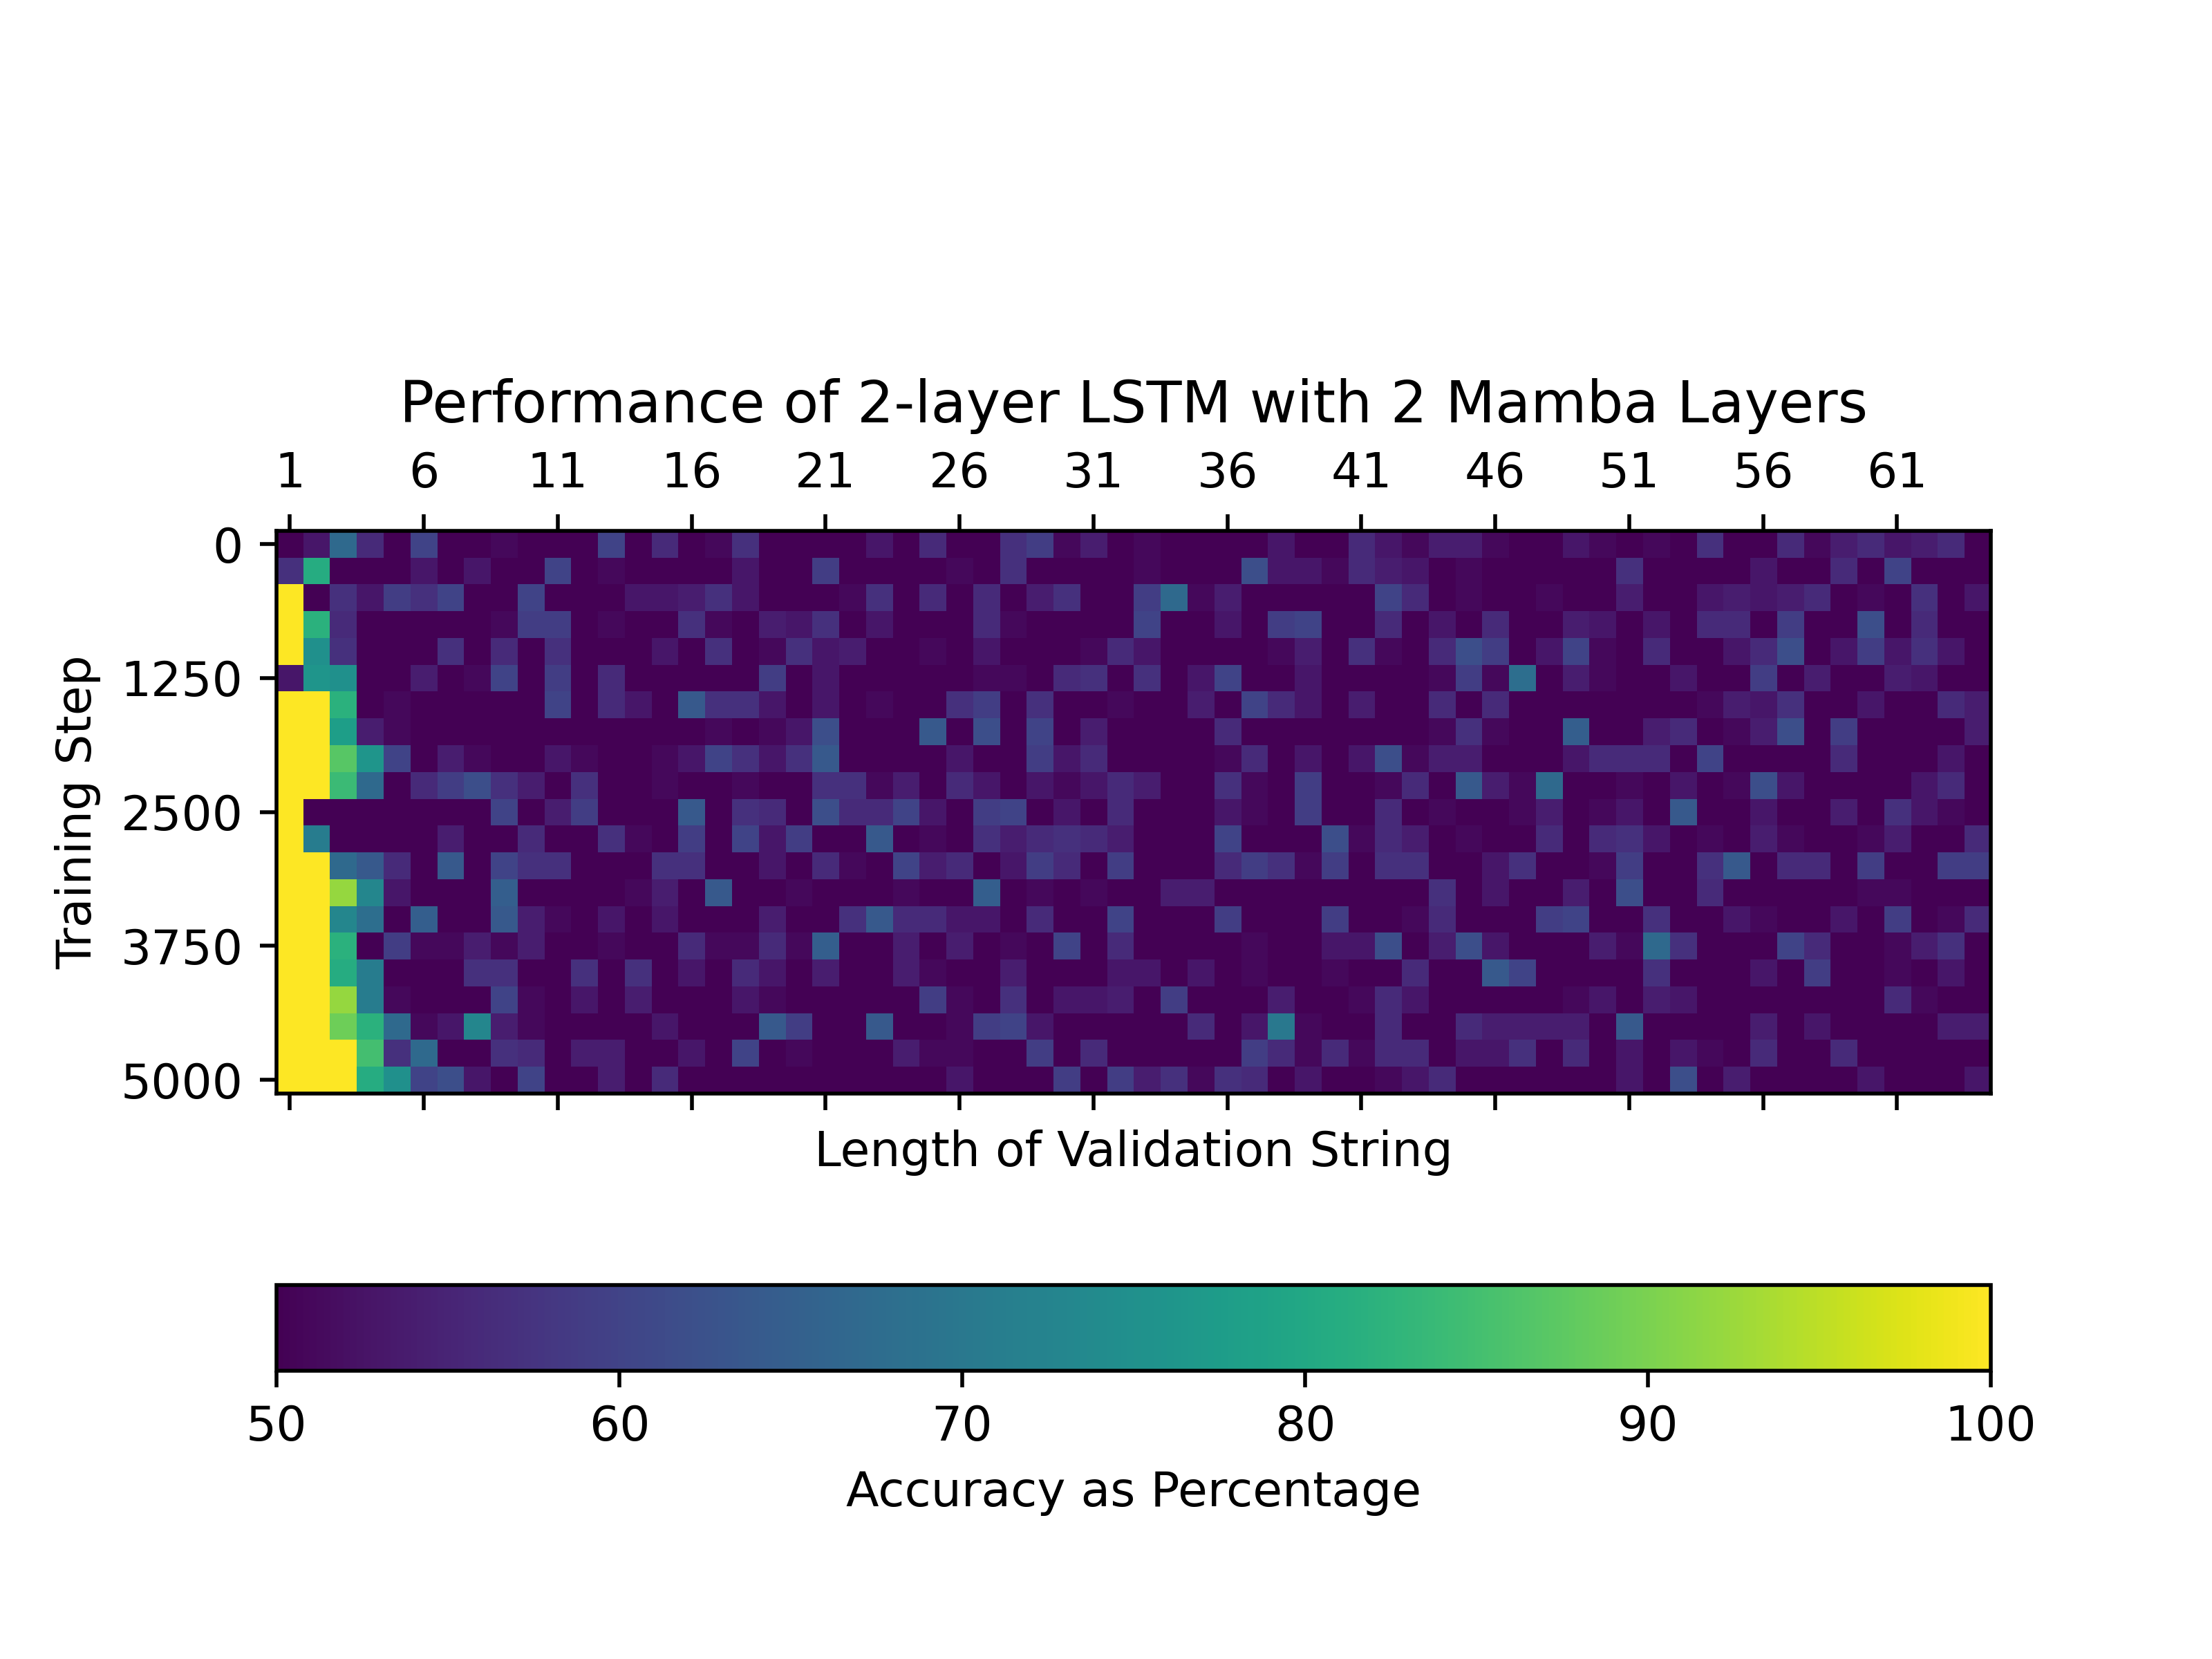
\includegraphics[width=0.8\textwidth]{figures/parity_lstm_False_4_2.png.png}
        \end{center}
    \end{subfigure}\begin{subfigure}{0.5\textwidth}
        \begin{center}
        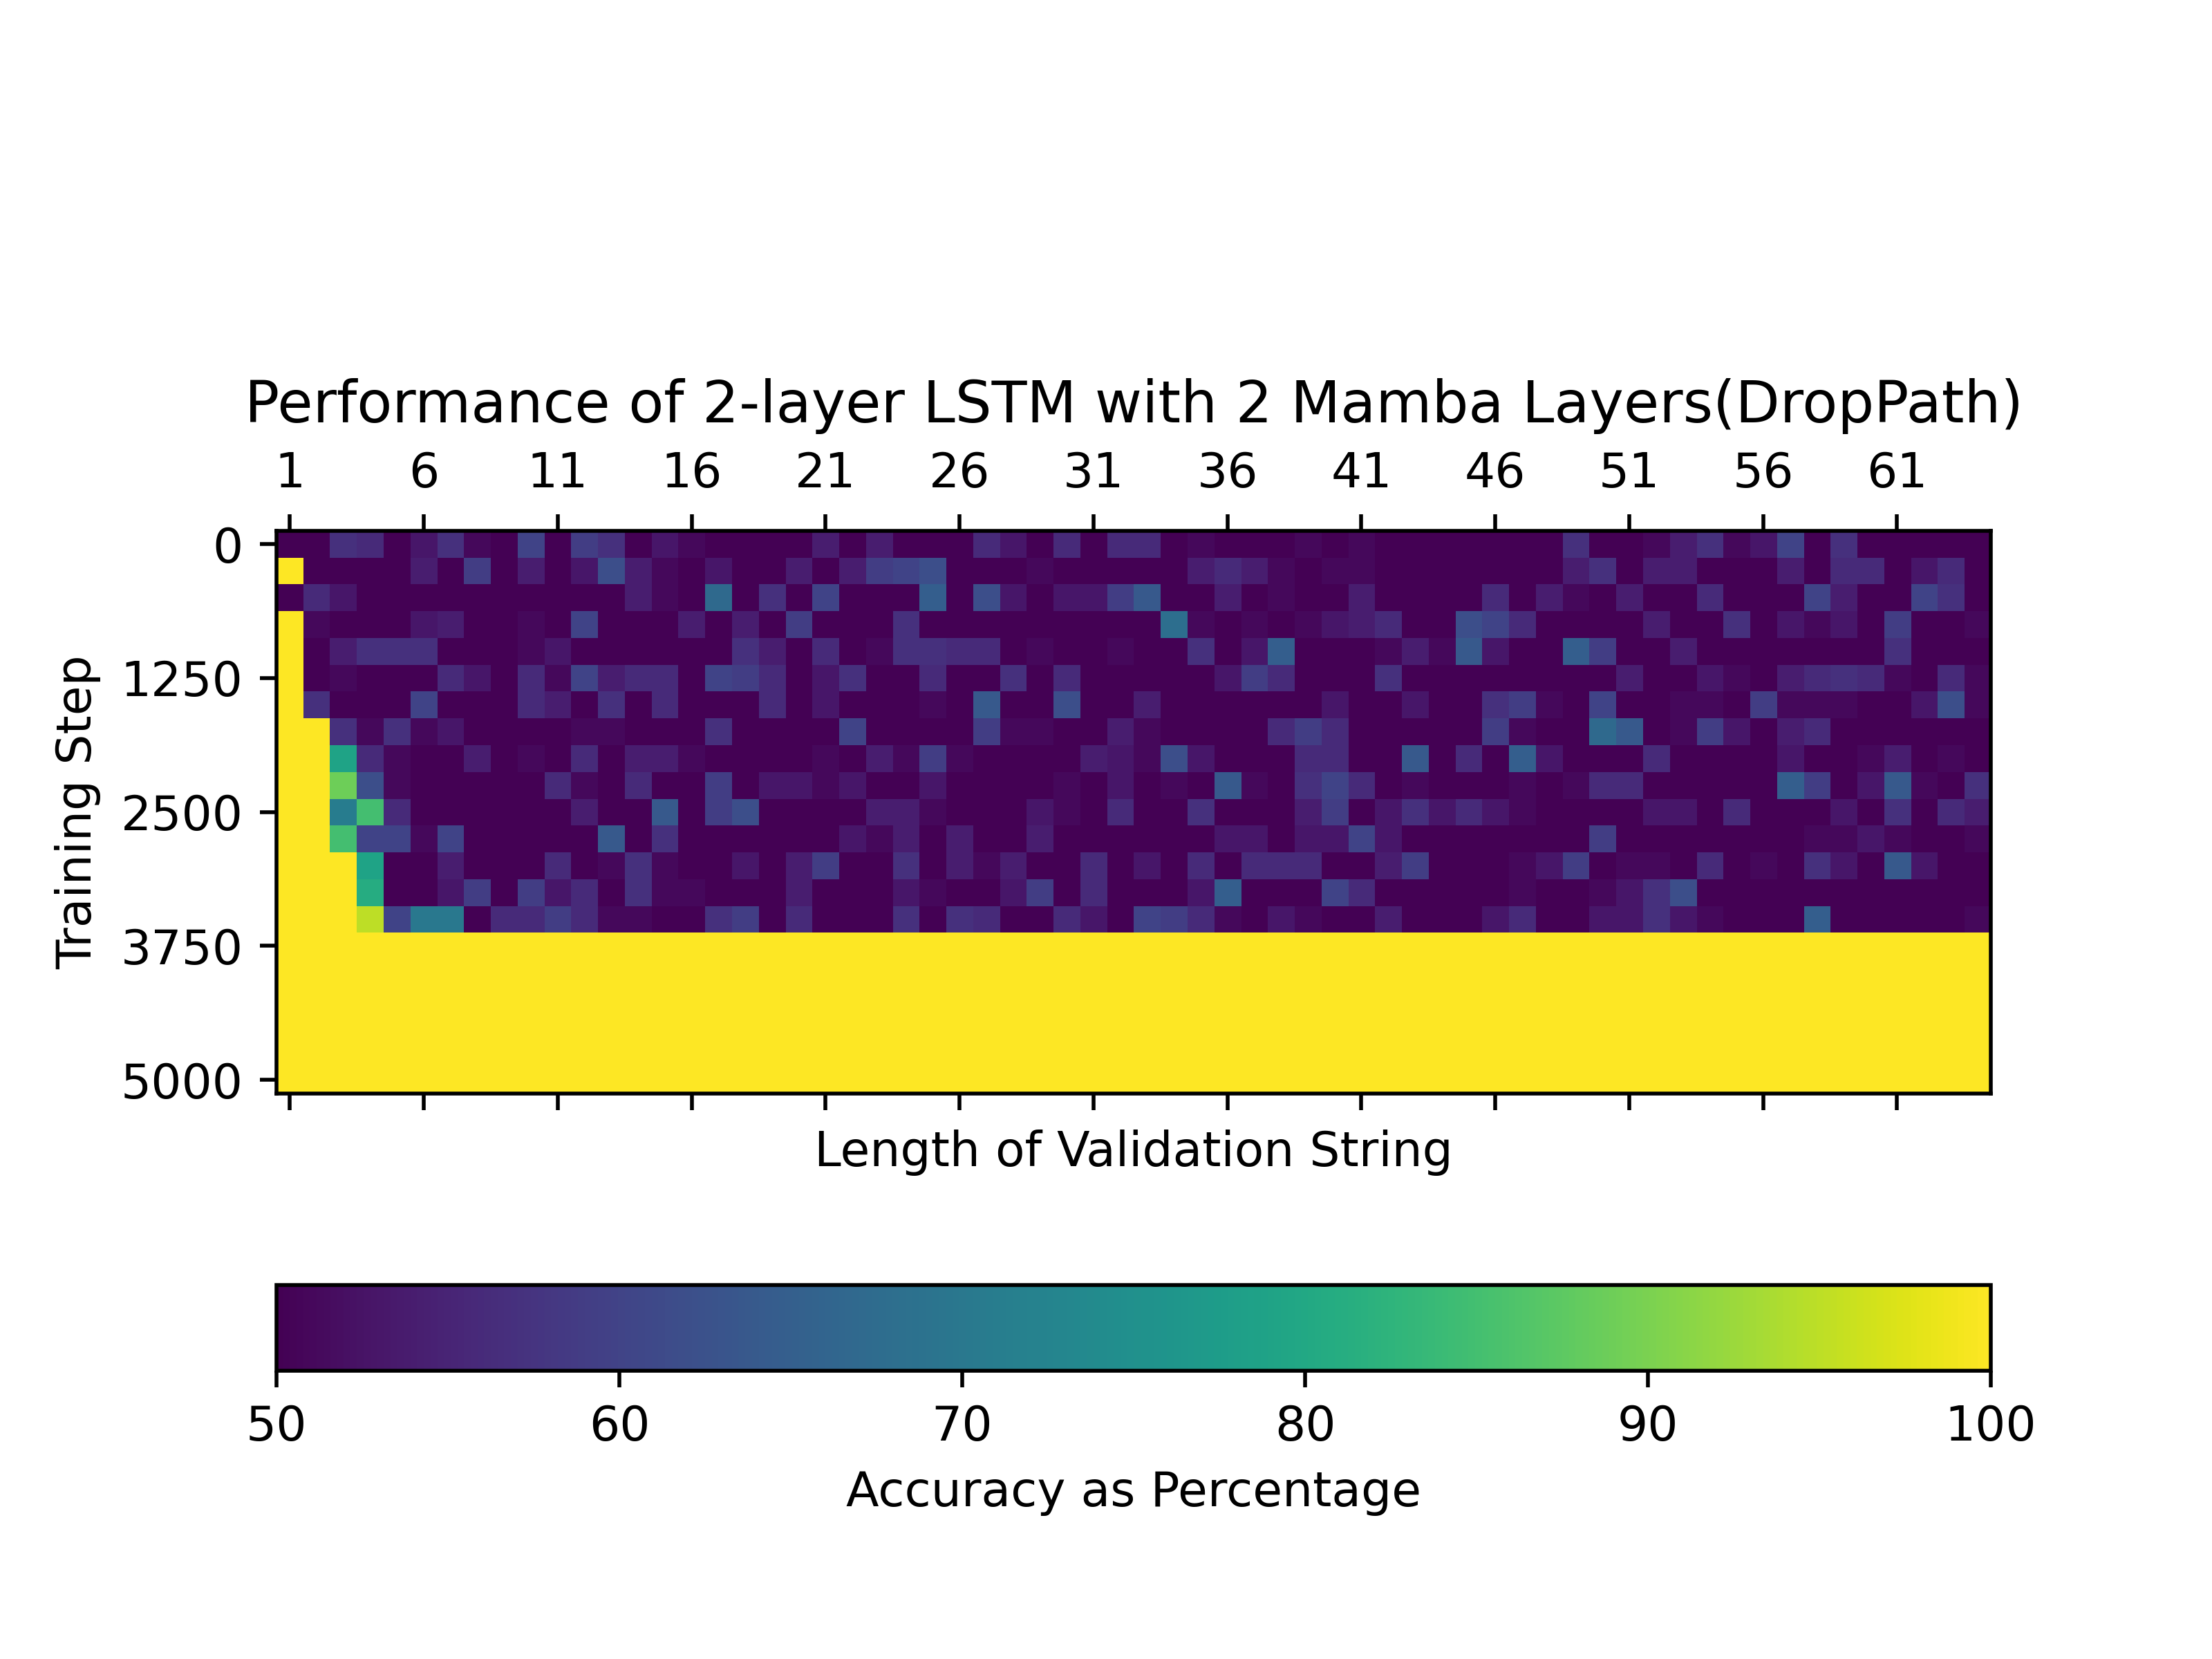
\includegraphics[width=0.8\textwidth]{figures/parity_lstm_True_4_2.png.png}
        \end{center}
    \end{subfigure}
    \begin{subfigure}{0.5\textwidth}
        \begin{center}
        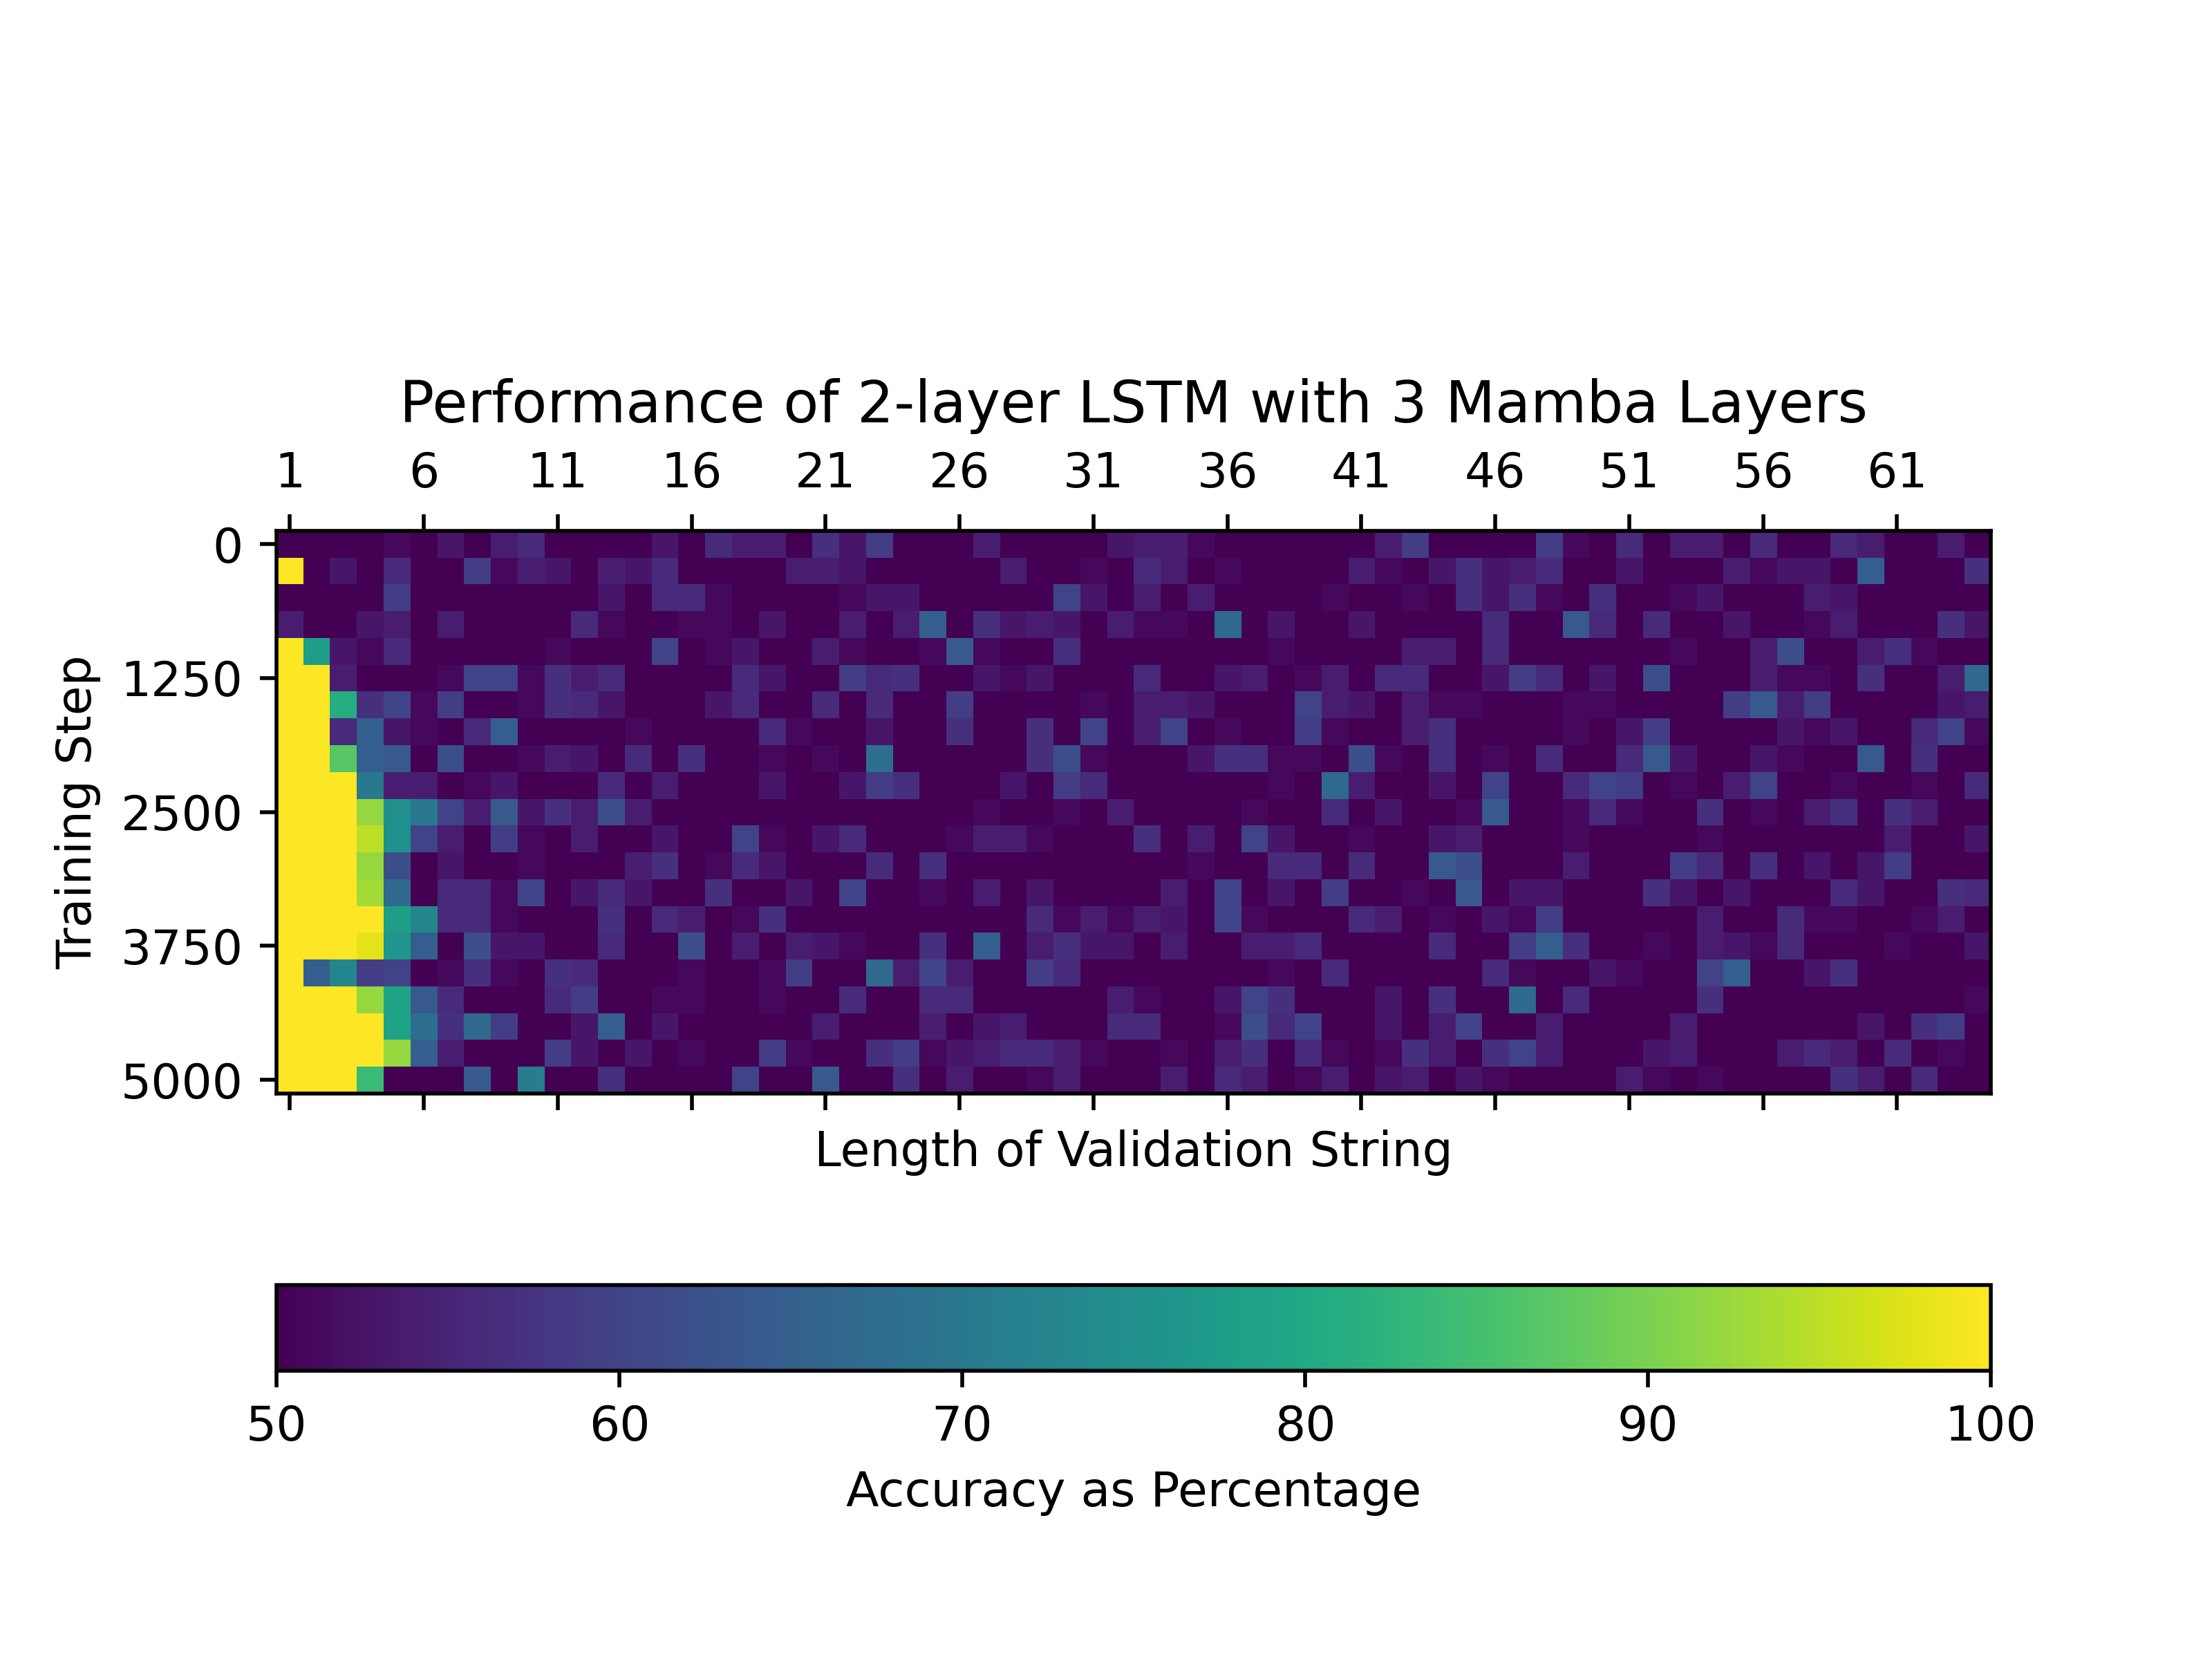
\includegraphics[width=0.8\textwidth]{figures/parity_lstm_False_5_1.png.png}
        \end{center}
    \end{subfigure}\begin{subfigure}{0.5\textwidth}
        \begin{center}
        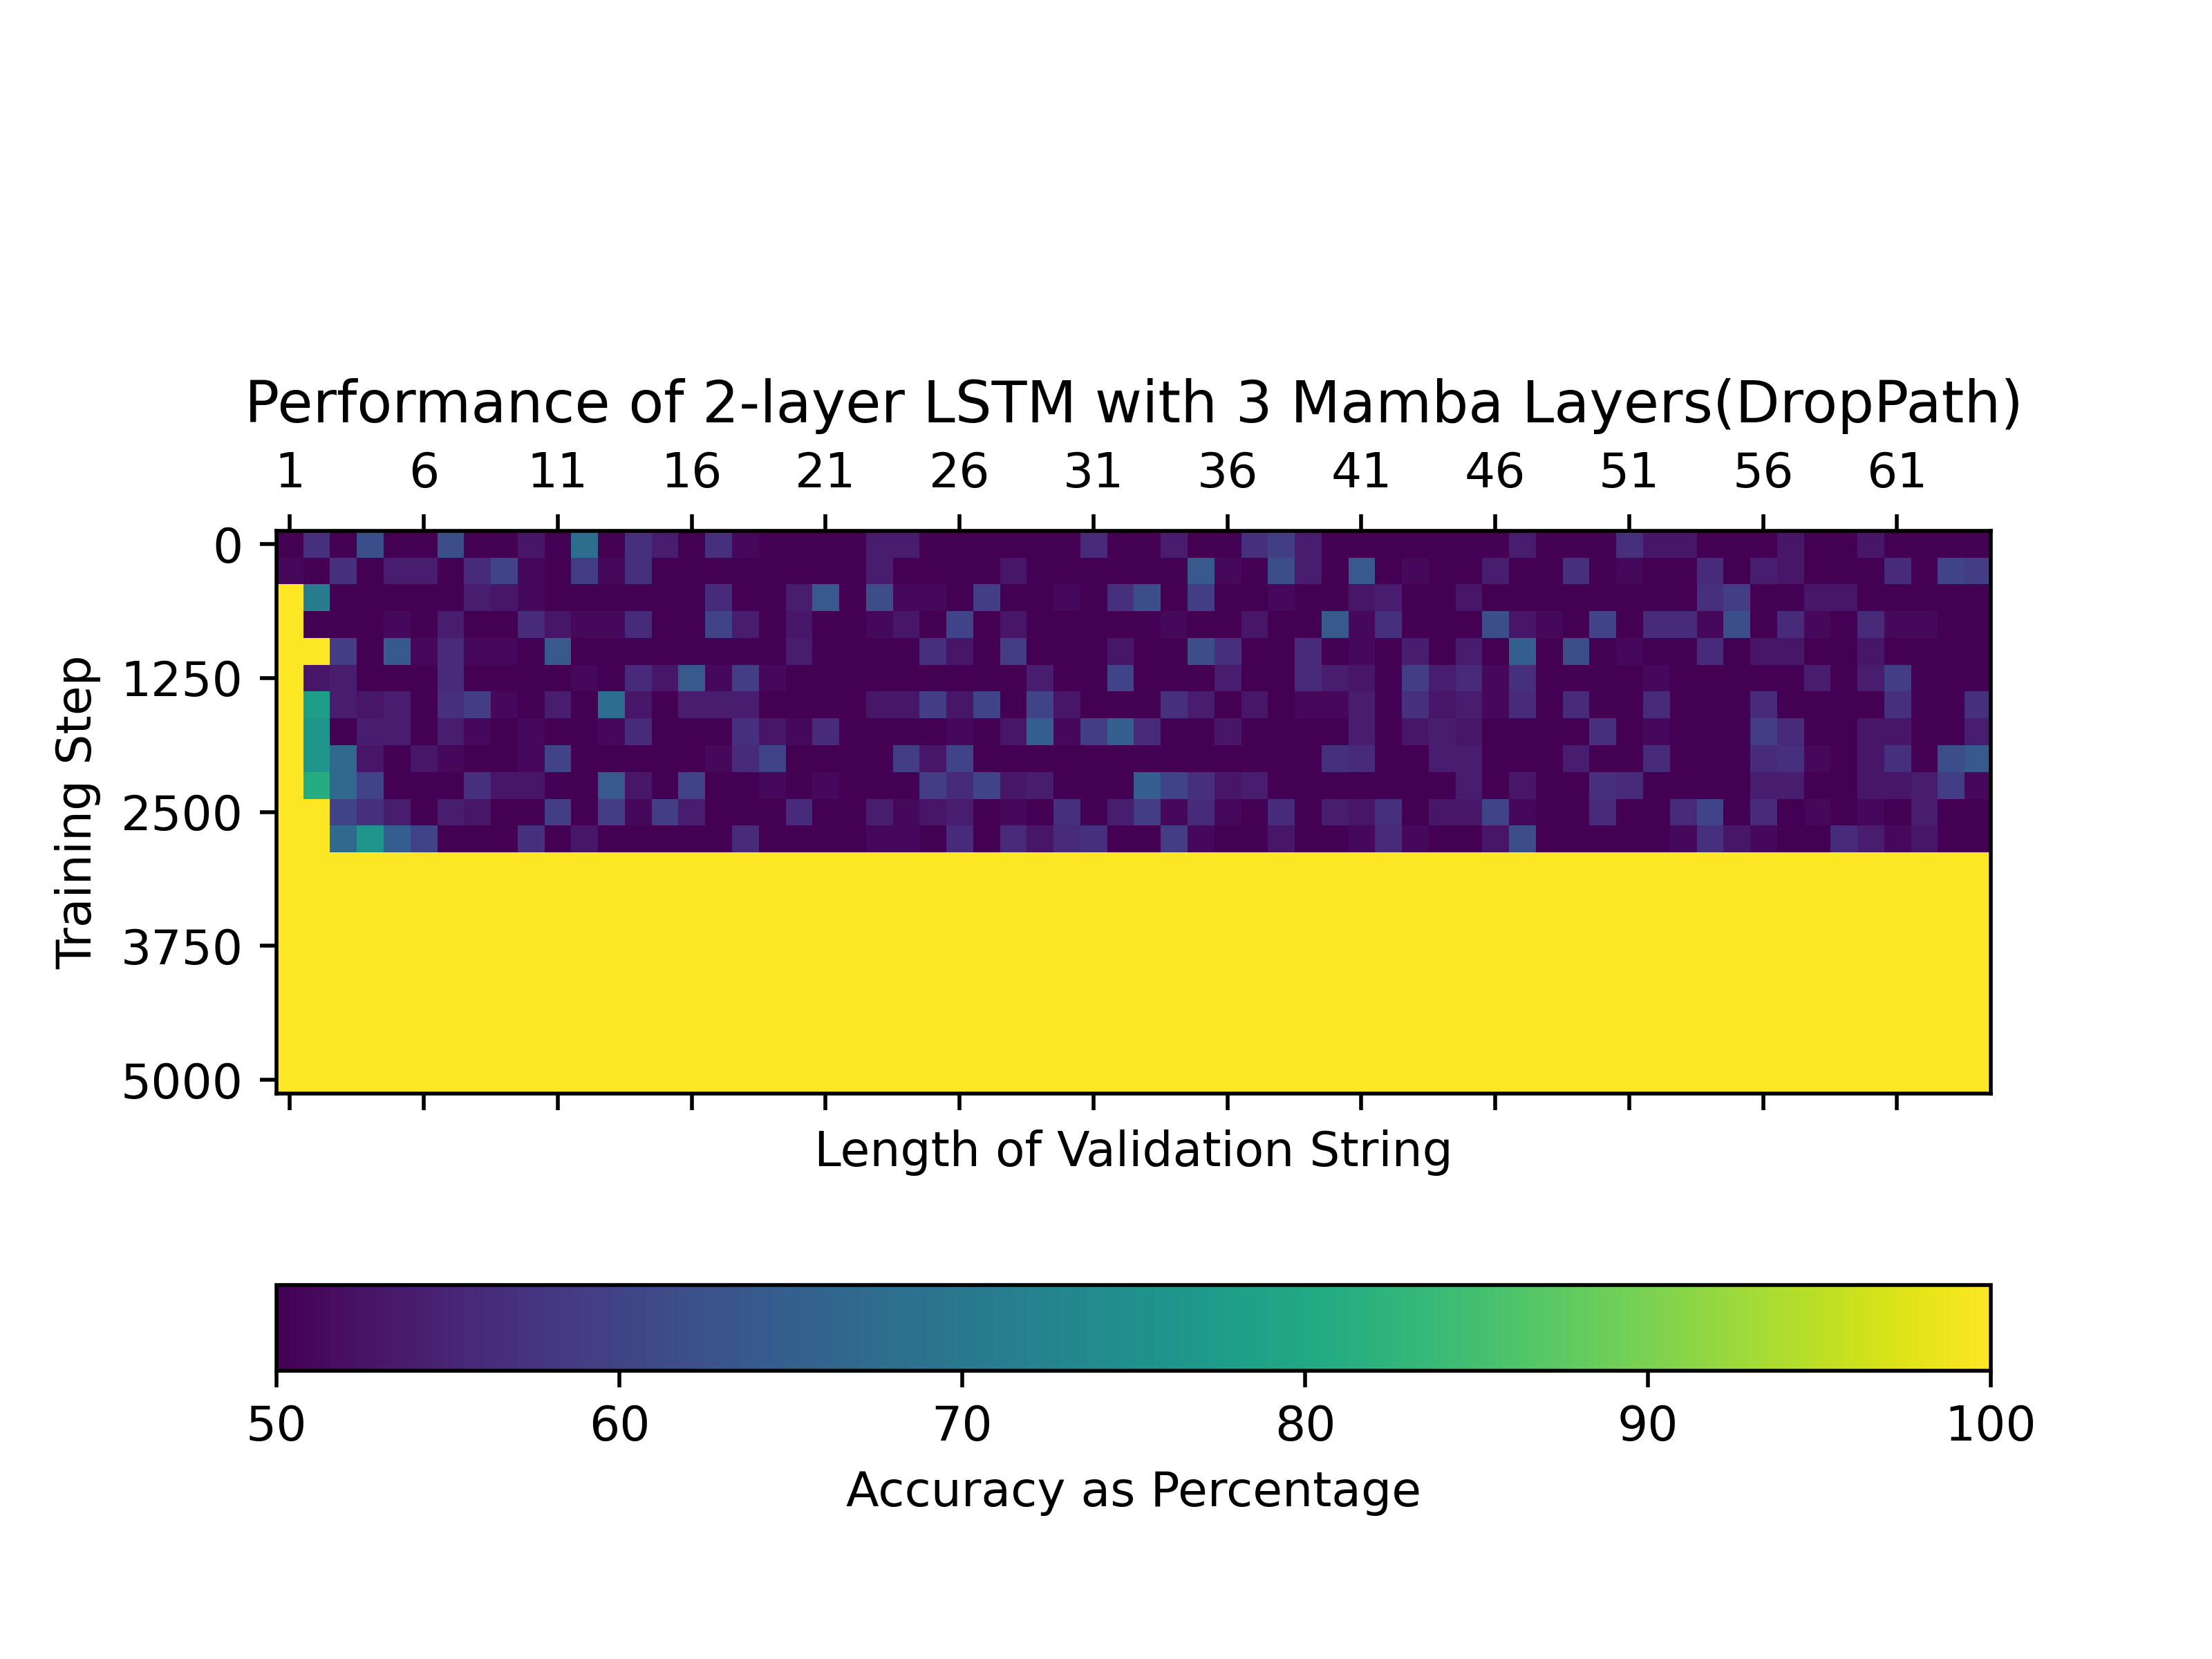
\includegraphics[width=0.8\textwidth]{figures/parity_lstm_True_5_1.png.png}
        \end{center}
    \end{subfigure}
    \begin{subfigure}{0.5\textwidth}
        \begin{center}
        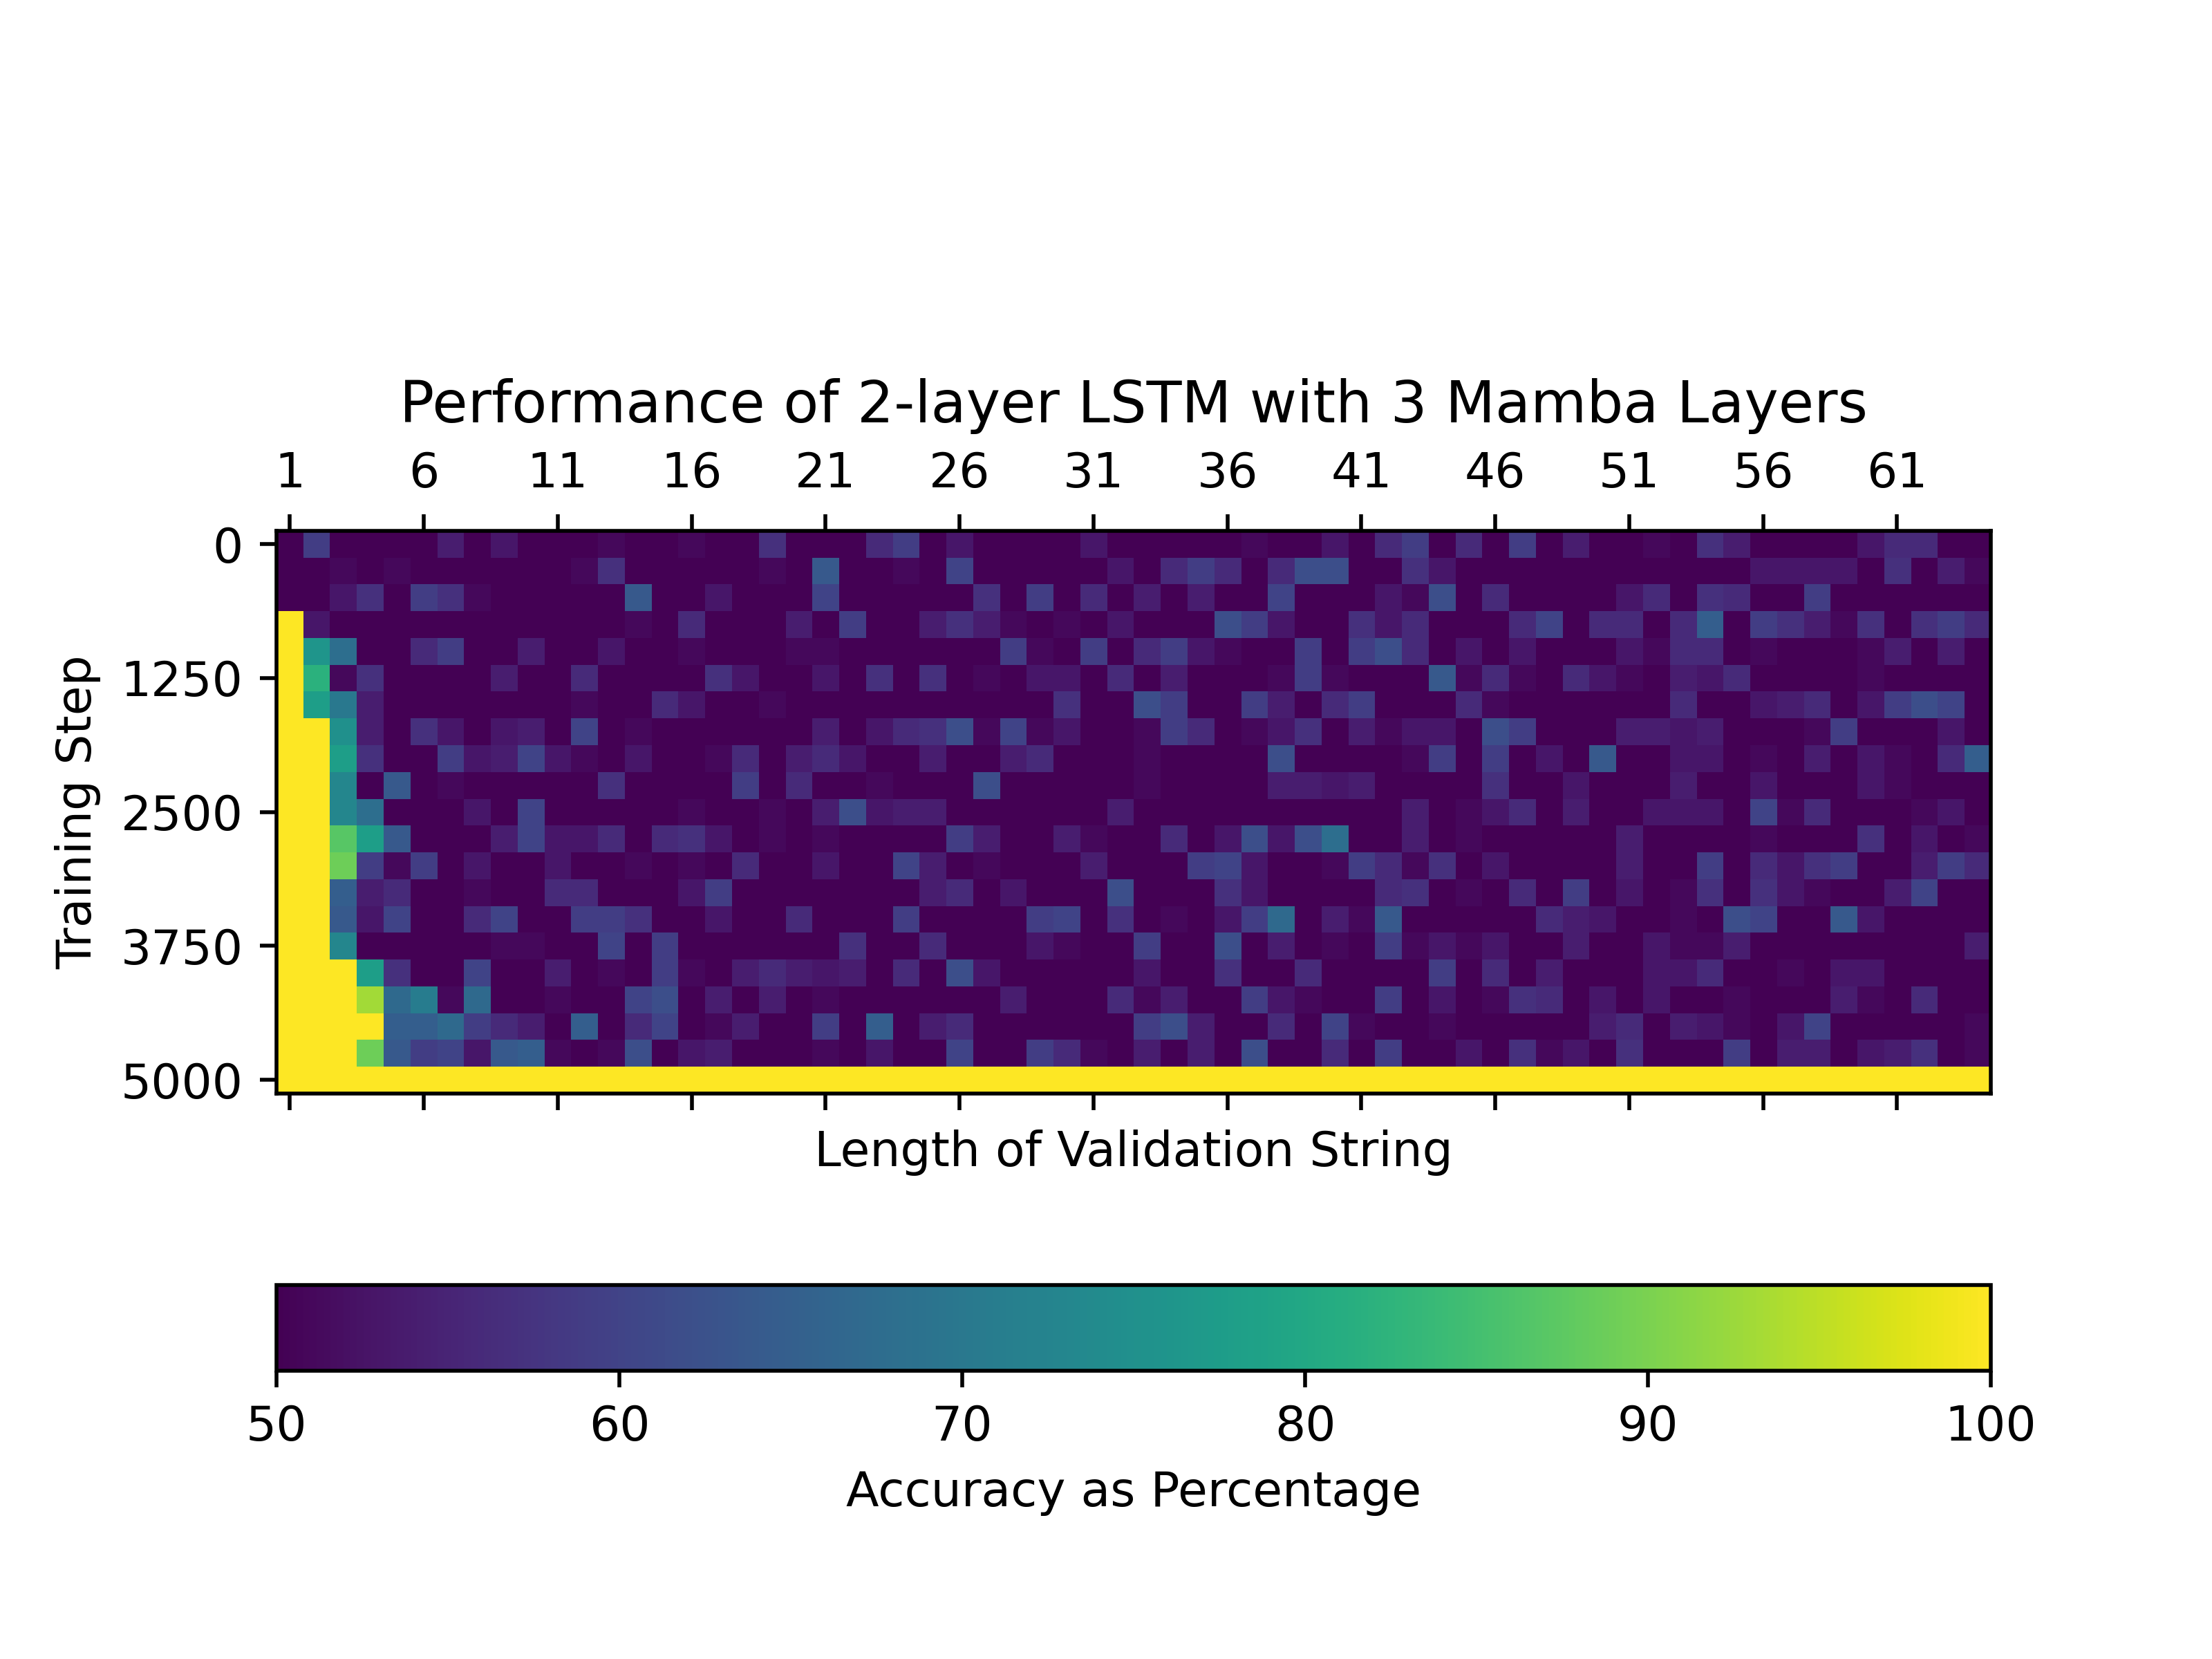
\includegraphics[width=0.8\textwidth]{figures/parity_lstm_False_5_2.png.png}
        \end{center}
    \end{subfigure}\begin{subfigure}{0.5\textwidth}
        \begin{center}
        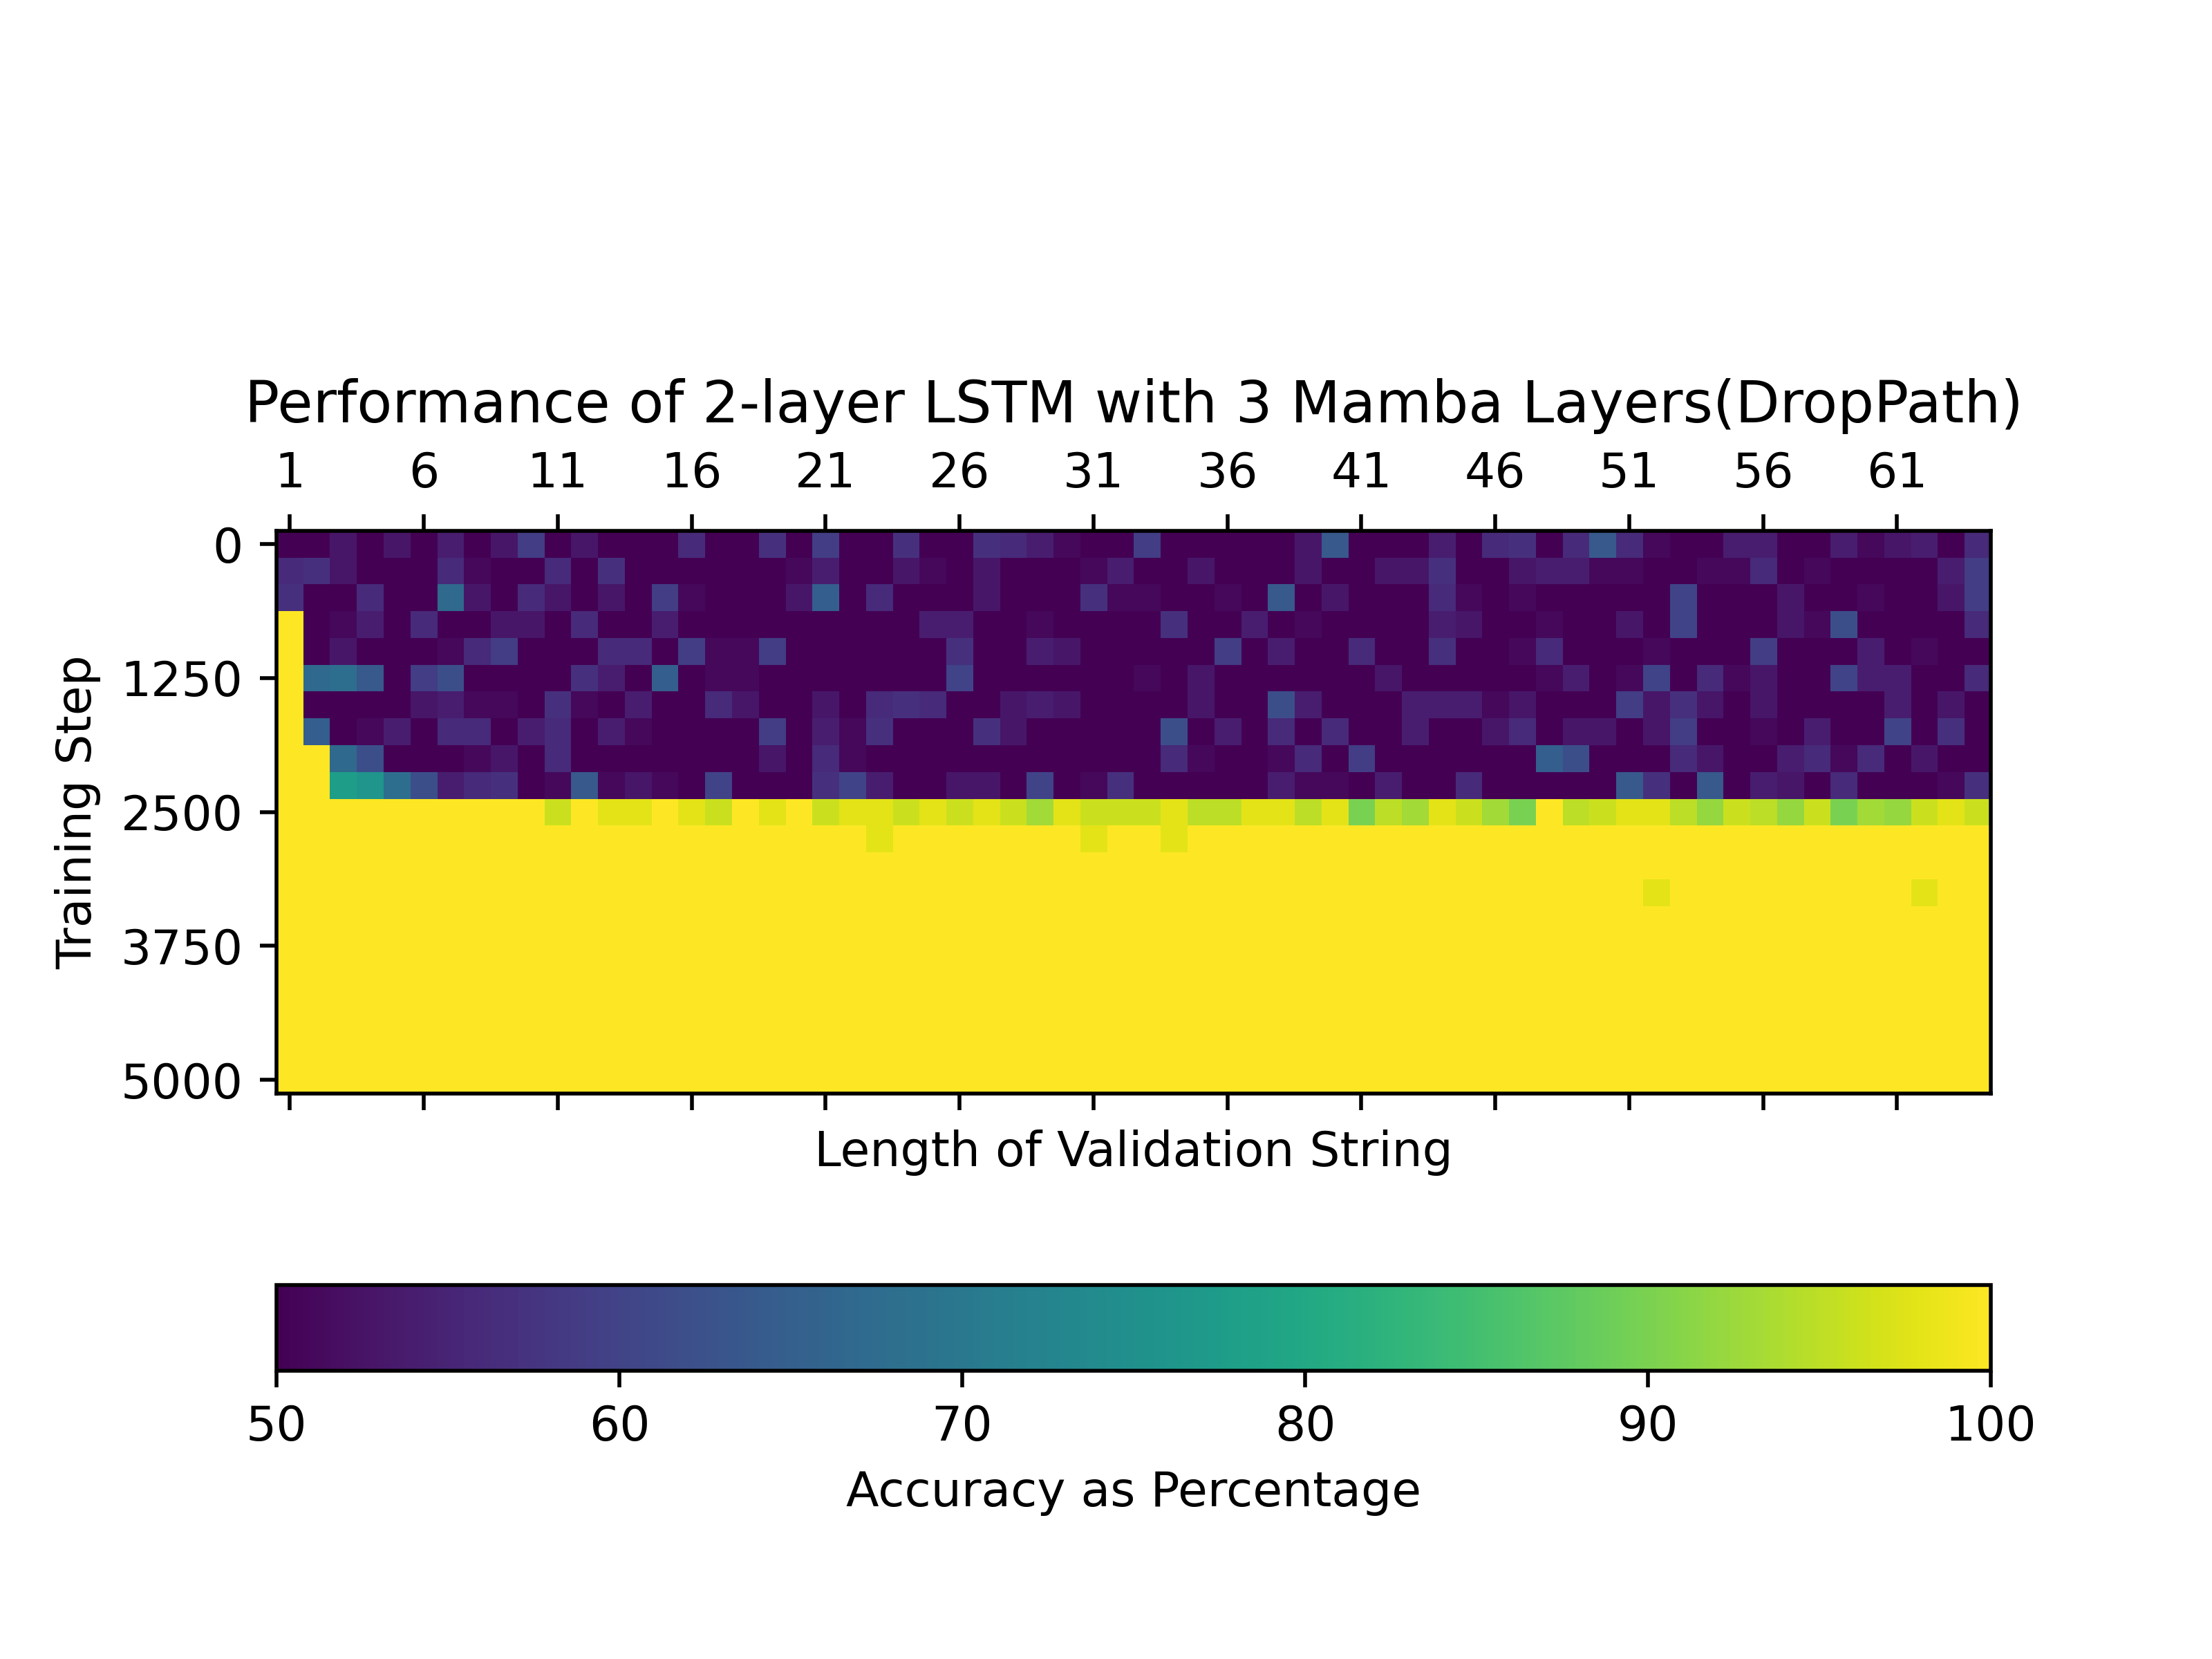
\includegraphics[width=0.8\textwidth]{figures/parity_lstm_True_5_2.png.png}
        \end{center}
    \end{subfigure}
    \caption{Results for parity}
    \label{droppathresults}
\end{figure}
as shown in Figure \ref{droppathresults}, all of the stacks with droppath
generalized within 5000 training steps, while only 3 of the 6 runs generalized
without Drop Path.

\subsection{Ability to recognize CFGs}

\textbf{Rationale} An interesting finding from the literature is that Mamba is
theoretically capable of recognizing some CFGs. For instance, SSMs are
theoretically capable of recognizing any Dyck language by implementing internal
counters.

An important component of many CFG-related operations is matching strings to
non-terminal symbols.




% explain that hyperparameters in original paper were unreasonable and risking
% overfitting
